\documentclass[11pt,a4paper]{article}

\usepackage[T1]{fontenc}
\usepackage[utf8]{inputenc}
\usepackage{lmodern}
\usepackage[margin=2.2cm]{geometry}
\usepackage{amsmath,amssymb}
\usepackage{graphicx}
\usepackage{booktabs}
\usepackage{array}
\usepackage{xcolor}
\usepackage{listings}
\usepackage{caption}
\usepackage{enumitem}
\usepackage{fancyhdr}
\usepackage[hidelinks]{hyperref}

\definecolor{fnoblue}{HTML}{3573B9}
\definecolor{donrose}{HTML}{B03A5B}
\definecolor{pfnogold}{HTML}{C98A00}
\definecolor{ink}{HTML}{222222}
\definecolor{muted}{HTML}{5B5B5B}
\definecolor{rule}{HTML}{D8D8D8}
\definecolor{codebg}{HTML}{F7F7F5}
\definecolor{codekw}{HTML}{1F5FA8}
\definecolor{codestr}{HTML}{7A6000}
\definecolor{codecom}{HTML}{6B6B6B}

\hypersetup{colorlinks=true,linkcolor=fnoblue,urlcolor=fnoblue}

\captionsetup{font=small,labelfont={bf,small}}

\lstset{
  language=Python,
  basicstyle=\ttfamily\footnotesize,
  keywordstyle=\color{codekw},
  stringstyle=\color{codestr},
  commentstyle=\color{codecom}\itshape,
  backgroundcolor=\color{codebg},
  frame=single,
  rulecolor=\color{rule},
  framesep=5pt,
  xleftmargin=6pt,
  breaklines=true,
  showstringspaces=false,
  columns=fullflexible,
  keepspaces=true,
}

\pagestyle{fancy}
\fancyhf{}
\lhead{\small\color{muted}Neural-operator wave simulations}
\rhead{\small\color{muted}\thepage}
\renewcommand{\headrulewidth}{0.4pt}

\newcommand{\relL}{relative $L_2$}

% Zero-width break opportunity, for long file names in typewriter text.
\newcommand{\bk}{\discretionary{}{}{}}
% Let TeX stretch interword space rather than run into the margin.
\emergencystretch=3em
\hbadness=10000

\title{\vspace{-1.4cm}\bfseries Neural-operator wave simulations\\[2mm]
\large FNO, DeepONet, and PFNO on the 1D elastic wave equation}
\author{\normalsize SciML Project --- wave equation operator baselines}
\date{\normalsize\today}

\begin{document}
\maketitle
\thispagestyle{fancy}

\noindent\fcolorbox{rule}{codebg}{%
\begin{minipage}{0.977\textwidth}
\small
\textbf{Summary.} Three neural operators are trained to map a heterogeneous
material profile and an initial pulse to the complete space--time displacement
field of the 1D elastic wave equation, supervised on finite-difference
solutions. An earlier version of this comparison produced animations that
showed noise rather than waves; the cause was diagnosed as a chronically
under-specified training set (16 samples, 12 epochs), not a defect in the
plotting. After enlarging the dataset to 512 samples, adding a one-cycle
learning-rate schedule, and increasing model capacity, validation error falls
from $81.9\%$ to $\mathbf{2.07\%}$ (FNO), $94.8\%$ to $\mathbf{4.26\%}$ (PFNO),
and $97.3\%$ to $\mathbf{14.43\%}$ (DeepONet). This document explains the
physics, the data, the architectures, the diagnosis, the visualization design,
and the code. A second arm (Section~\ref{sec:forced}) replaces the initial pulse
with a Ricker point source and reports initial- and boundary-condition
residuals, which turn out to need careful reading: the worst model scores the
best boundary residual, because a collapsed field satisfies the condition
trivially. Section~\ref{sec:pinn} then promotes those residuals to training
losses: FNO improves on every axis, PFNO is unmoved, and DeepONet gets worse ---
for an underfitting model the constraints pull toward the trivial solution.
\end{minipage}}

\vspace{4mm}
{\small\tableofcontents}
\clearpage

%==============================================================
\section{What the simulations show}

Each animation in \texttt{simulations/} covers one \textbf{held-out} velocity
model. FNO, DeepONet, and PFNO each receive the material profile and the
initial pulse, and predict the \emph{entire} displacement field $u(x,t)$ in a
single forward pass --- no time stepping and no PDE solve at inference. The
animation then sweeps a cursor through the predicted time slices and compares
them against the finite-difference (FD) solution of the same problem.

The purpose is to test \emph{generalization}. These velocity models were never
seen in training. A model that has genuinely learned the solution operator must
reproduce the correct wave speed, the correct reflection and transmission
amplitudes at each material interface, and the correct arrival times, for a
material it has never encountered.

Four animations are provided, one per material family. Each is the
\textbf{median-error} sample of its family, not the best case.

\begin{center}
\small
\begin{tabular}{llrrr}
\toprule
\textbf{File} & \textbf{Material} & \textbf{FNO} & \textbf{DeepONet} & \textbf{PFNO}\\
\midrule
\texttt{\dots sample\_75\_homogeneous.gif} & homogeneous     & $0.13\%$ & $4.29\%$  & $0.55\%$\\
\texttt{\dots sample\_275\_two\_layer.gif} & two-layer       & $1.27\%$ & $8.20\%$  & $2.90\%$\\
\texttt{\dots sample\_353\_smooth.gif}     & smooth          & $0.63\%$ & $10.70\%$ & $2.43\%$\\
\texttt{\dots sample\_398\_layered.gif}    & layered (3--7)  & $4.67\%$ & $24.91\%$ & $10.63\%$\\
\bottomrule
\end{tabular}
\end{center}

\noindent Percentages are \relL{} error against the FD reference for that sample.

A further nine animations cover the three real velocity models, in
\texttt{simulations/real/} --- see \S\ref{sec:realgifs}. Four more in
\texttt{simulations/source\_term/} belong to the forced arm, and
\texttt{simulations/superseded\_undertrained/} keeps three from the original
under-trained run.

%==============================================================
\section{How to read a frame}

The figure is two rows by four columns.

\begin{center}
\small
\begin{tabular}{|>{\raggedright\arraybackslash}p{3.1cm}|>{\raggedright\arraybackslash}p{3.1cm}|>{\raggedright\arraybackslash}p{3.1cm}|>{\raggedright\arraybackslash}p{3.1cm}|}
\hline
velocity model $c(x)$ & FNO vs FD ref & DeepONet vs FD ref & PFNO vs FD ref\\
\hline
FD reference field $u(x,t)$ & FNO prediction & DeepONet prediction & PFNO prediction\\
\hline
\end{tabular}
\end{center}

\begin{itemize}[leftmargin=*,itemsep=2pt]
\item \textbf{Top left} --- the wave speed $c(x)=\sqrt{E(x)/\rho(x)}$ for this
sample, with the current time beside it. This is the \emph{input} the operators
are conditioned on; everything else in the figure follows from it.
\item \textbf{Top row, columns 2--4} --- displacement $u(\cdot,t)$ at the current
time. The thick grey curve is the FD reference; the coloured curve is the
model. Where the colour hides the grey, the model is correct. The title gives
the \relL{} for the whole field, not just that frame.
\item \textbf{Bottom left} --- the FD reference field over the full $(x,t)$
domain, with a horizontal cursor at the current time.
\item \textbf{Bottom row, columns 2--4} --- each model's predicted field on the
\emph{same} colour scale, so panels are directly comparable.
\end{itemize}

\paragraph{Reading the space--time panels.} Time runs upward. A wave at constant
speed traces a straight line of slope $1/c$. The initial pulse at $t=0$, $x=0$
splits into a left-going and a right-going wave --- the characteristic ``V''.
Where $c(x)$ changes the V \emph{kinks} (refraction changes the slope) and sheds
a fainter secondary line travelling the other way (reflection). The layered
sample shows this most clearly; the homogeneous sample is a clean straight V
with no reflections at all.

\begin{figure}[htbp]
\centering
\makebox[\textwidth][c]{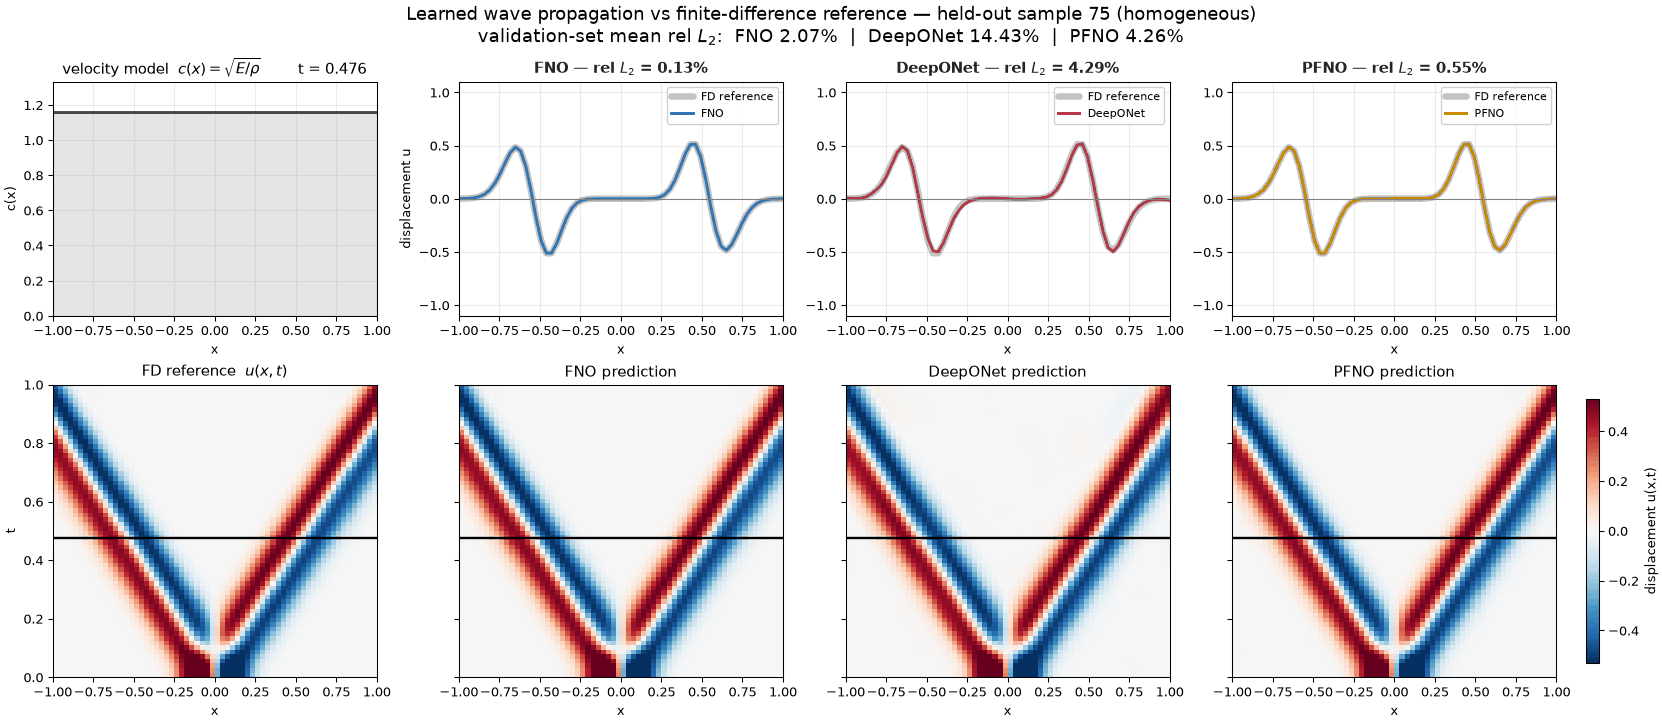
\includegraphics[width=1.18\textwidth]{figures/frame_homogeneous.png}}
\caption{Homogeneous medium, $c$ constant. A clean straight V with no
reflections; FNO and PFNO are visually indistinguishable from the reference
($0.13\%$ and $0.55\%$).}
\end{figure}

\begin{figure}[htbp]
\centering
\makebox[\textwidth][c]{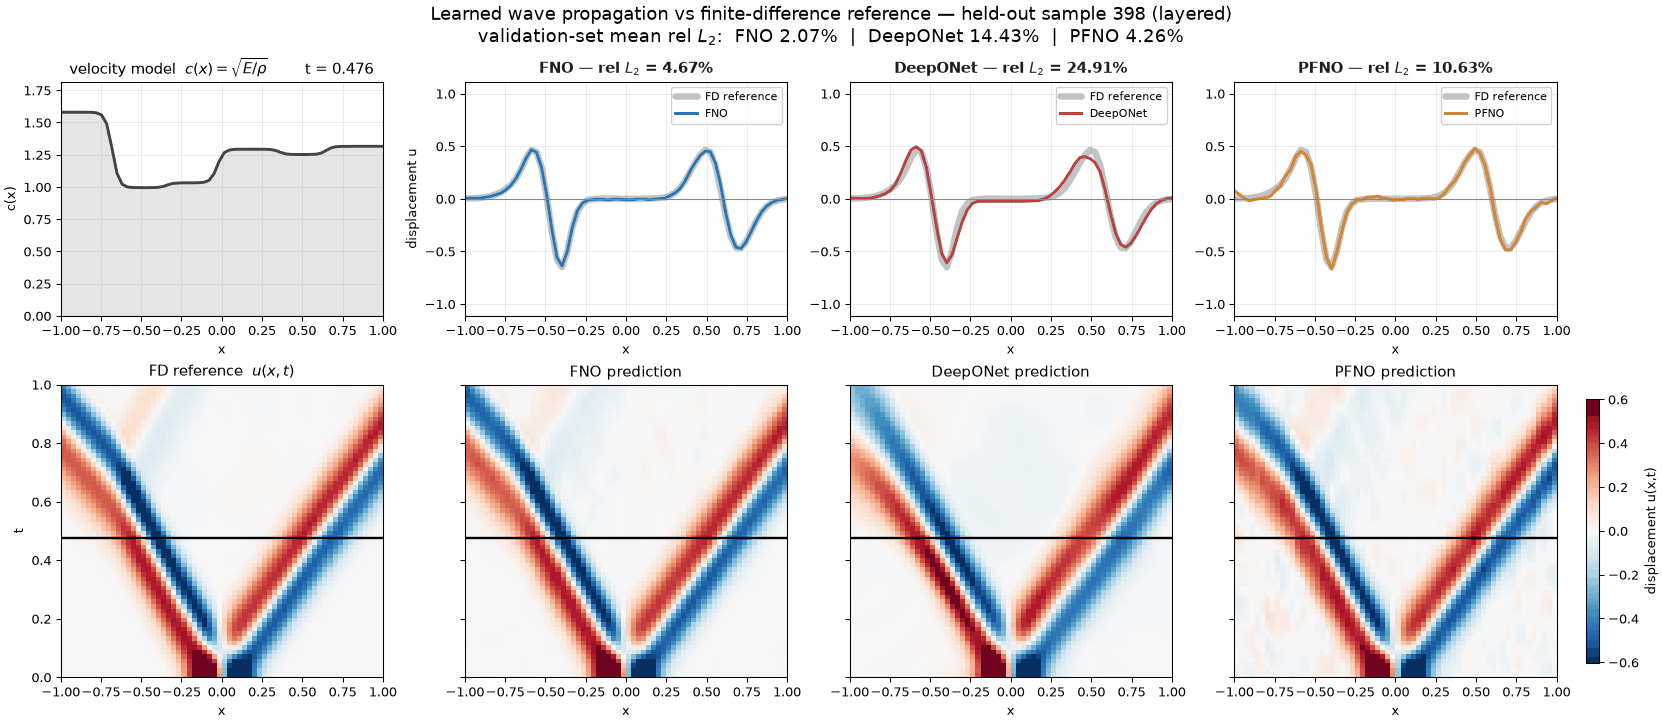
\includegraphics[width=1.18\textwidth]{figures/frame_layered.png}}
\caption{Layered medium, the hardest family. Every interface splits the wave,
producing the secondary lines visible in the space--time panels. DeepONet's
amplitude deficit against the grey reference is clearly visible in the top row.}
\end{figure}

\clearpage

%==============================================================
\section{The physics being learned}

The governing equation is the 1D elastic wave equation in \textbf{conservative
form},
\begin{equation}
\rho(x)\,u_{tt} \;=\; \frac{\partial}{\partial x}\!\left[E(x)\,u_x\right],
\qquad x\in[-1,1],\quad t\in[0,1],
\end{equation}
with $E(x)$ the stiffness and $\rho(x)$ the density. The local wave speed is
$c(x)=\sqrt{E(x)/\rho(x)}$.

The conservative form matters. Expanding gives
\begin{equation}
\rho\,u_{tt} \;=\; E\,u_{xx} + E_x\,u_x ,
\end{equation}
so the naive $u_{tt}=c(x)^2u_{xx}$ drops the $E_x u_x$ term --- precisely the
term that sets reflection and transmission amplitudes at a material interface.
In layered media that approximation gets the physics wrong, so both the FD
reference and the wider project use the conservative form throughout.

\paragraph{Initial conditions.} A Gaussian-derivative pulse normalized to unit
peak, with zero initial velocity,
\begin{equation}
f(x)=\frac{\partial}{\partial x}\exp\!\left(-\tfrac12\left(\tfrac{x-x_0}{\sigma_g}\right)^{2}\right)
\Big/ \max|\cdot| ,
\qquad g(x)=u_t(x,0)=0,
\end{equation}
with $\sigma_g=0.1$ and $x_0=0$ fixed for every sample (hence \texttt{fixedic}
in the dataset filename). Because the initial velocity is zero, the pulse splits
symmetrically into two counter-propagating waves of roughly half amplitude each
--- which is why the $t=0$ frame is about $1.8\times$ taller than everything
after it. This has direct consequences for the colour scale
(Section~\ref{sec:viz}).

\paragraph{Boundary conditions.} First-order absorbing (radiation) conditions,
$u_t \mp c\,u_x = 0$ at the left/right boundary, so waves leave the domain
without reflecting.

\paragraph{The FD reference.} \texttt{wave/fd\_solver.py} is an explicit
second-order leapfrog scheme in flux form. Two details are load-bearing:

\begin{itemize}[leftmargin=*,itemsep=2pt]
\item \textbf{Harmonic-mean interface stiffness},
$E_{i+1/2} = 2E_iE_{i+1}/(E_i+E_{i+1})$, which preserves correct transmission
and reflection across a jump in $E$.
\item \textbf{Mur discretization} of the absorbing boundaries,
$u_0^{n+1}=u_1^{n}+\beta\,(u_1^{n+1}-u_0^{n})$ with
$\beta=(c\,\Delta t-\Delta x)/(c\,\Delta t+\Delta x)$. The apparently natural
centred-time / one-sided-space discretization is \emph{unconditionally
unstable} --- round-off grows exponentially from the boundary.
\end{itemize}

The solver chooses its own $\Delta t$ from the CFL condition; the generator then
interpolates onto the uniform 64-point output time grid.

%==============================================================
\section{The dataset}

\texttt{operator\_data/\bk wave\_operator\bk\_fixedic\bk\_n512\bk\_nx64\bk\_nt64\bk\_t1\bk\_seed42.npz}

\medskip\noindent
512 samples on a $64\times64$ $(x,t)$ grid, $x\in[-1,1]$, $t\in[0,1]$, seed 42,
CFL $0.35$. Generation takes about two seconds.

\paragraph{Velocity models.} $\rho(x)=1$ everywhere, so $c(x)=\sqrt{E(x)}$. Each
sample draws one of four $E(x)$ families uniformly:

\begin{center}
\small
\begin{tabular}{llp{9.2cm}}
\toprule
\textbf{Family} & \textbf{Count} & \textbf{Construction}\\
\midrule
\texttt{homogeneous} & 125 & constant, $E\sim U(0.7,2.2)$\\
\texttt{two\_layer}  & 130 & tanh-smoothed step, left $U(0.7,1.5)$ to right $U(1.0,2.5)$, interface at $U(-0.45,0.45)$, width $U(0.015,0.06)$\\
\texttt{layered}     & 131 & 3--7 tanh-blended layers, values $U(0.7,2.5)$, boundaries jittered by $\mathcal{N}(0,0.04)$\\
\texttt{smooth}      & 126 & base $U(0.9,1.4)$ plus three sinusoids (freq.\ 1,2,3; amp.\ $U(-0.18,0.18)$), clipped to $[0.55,2.5]$\\
\bottomrule
\end{tabular}
\end{center}

\noindent Across the 512 samples the realized wave speeds span
$c\in[0.78,1.58]$.

\begin{lstlisting}
def sample_material_profile(rng, x):
    kind = rng.choice(["homogeneous", "two_layer", "layered", "smooth"])
    rho = np.ones_like(x, dtype=np.float64)

    if kind == "homogeneous":
        E = np.full_like(x, rng.uniform(0.7, 2.2), dtype=np.float64)
    elif kind == "two_layer":
        left, right = rng.uniform(0.7, 1.5), rng.uniform(1.0, 2.5)
        boundary, width = rng.uniform(-0.45, 0.45), rng.uniform(0.015, 0.06)
        alpha = 0.5 * (1.0 + np.tanh((x - boundary) / width))
        E = left * (1.0 - alpha) + right * alpha
    elif kind == "layered":
        n_layers = int(rng.integers(3, 8))
        values = rng.uniform(0.7, 2.5, size=n_layers)
        boundaries = np.linspace(x.min(), x.max(), n_layers + 1)[1:-1]
        boundaries += rng.normal(scale=0.04, size=boundaries.shape)
        width = rng.uniform(0.015, 0.05)
        E = np.full_like(x, values[0], dtype=np.float64)
        for value, boundary in zip(values[1:], boundaries):
            alpha = 0.5 * (1.0 + np.tanh((x - boundary) / width))
            E = E * (1.0 - alpha) + value * alpha
    else:  # smooth
        E = np.full_like(x, rng.uniform(0.9, 1.4), dtype=np.float64)
        for freq in (1, 2, 3):
            E += rng.uniform(-0.18, 0.18) * np.sin(
                freq * np.pi * (x + 1.0) + rng.uniform(0.0, 2.0 * np.pi))
        E = np.clip(E, 0.55, 2.5)

    return E.astype(np.float64), rho, str(kind)
\end{lstlisting}

\paragraph{Tensor layout.} Inputs are (sample, channel, $x$, $t$) with five
channels $[E,\rho,g,x,t]$; the three profiles are broadcast along the time axis
and $x$, $t$ are coordinate meshes. Outputs are (sample, 1, $x$, $t$).

\begin{center}\small\ttfamily
inputs : (512, 5, 64, 64) \quad channels [E(x), rho(x), g(x), x, t]\\
outputs: (512, 1, 64, 64) \quad u(x,t)
\end{center}

%==============================================================
\section{The operator-learning problem}

The models learn the map
\begin{equation}
\bigl[E(x),\ \rho(x),\ g(x),\ x,\ t\bigr] \;\longmapsto\; u(x,t),
\end{equation}
supervised on FD solutions. This is \emph{supervised} operator learning: there
is no PDE residual in the loss, unlike the PINN/KAN side of this repository. The
network never sees the equation, only input/output pairs.

\paragraph{Split.} $20\%$ validation via a seeded permutation: \textbf{410
train, 102 validation}. All reported numbers are on the validation set, and all
four animated samples are validation samples.

\paragraph{Normalization.} Per-channel mean/standard deviation for inputs and a
single scalar mean/standard deviation for the output, both computed on the
\textbf{training split only} so no validation statistics leak.

\begin{lstlisting}
x_mean = X[train_idx].mean(dim=(0, 2, 3), keepdim=True)
x_std  = X[train_idx].std(dim=(0, 2, 3), keepdim=True).clamp_min(1e-6)
y_mean = Y[train_idx].mean()
y_std  = Y[train_idx].std().clamp_min(1e-6)
\end{lstlisting}

\paragraph{Loss and metric.} Training minimizes MSE in normalized space. The
reported metric is \relL{} \emph{in physical units}, computed per sample and
averaged:
\begin{equation}
\text{rel}\ L_2 \;=\; \frac{\lVert \hat{u}-u\rVert_2}{\lVert u\rVert_2}.
\end{equation}
This metric has a useful calibration property: \textbf{a model that outputs all
zeros scores about $100\%$}. Anything near $100\%$ has learned nothing. The
state with the best validation MSE across all epochs is kept, not the final
state.

%==============================================================
\section{The three architectures}

\subsection{FNO --- 2D Fourier Neural Operator}

Lift the five input channels to \texttt{width} channels with a $1\times1$
convolution, apply blocks of $\mathrm{GELU}(\text{spectral}(z)+\text{local}(z))$,
then project to one output channel. The spectral layer takes a 2D real FFT over
$(x,t)$, multiplies the lowest $\text{modes}_x\times\text{modes}_t$ coefficients
by learned complex weights, zeroes the rest, and inverts.

\begin{lstlisting}
def forward(self, x):
    batch, _, nx_local, nt_local = x.shape
    x_ft = torch.fft.rfft2(x, norm="ortho")
    out_ft = torch.zeros(batch, self.weight_pos.shape[1], nx_local,
                         nt_local // 2 + 1, dtype=torch.cfloat, device=x.device)
    mx = min(self.modes_x, nx_local)
    mt = min(self.modes_t, nt_local // 2 + 1)
    # Both ends of the x axis are kept: rfft2 is only half-spectrum in t.
    out_ft[:, :, :mx, :mt]  = self.complex_mul(x_ft[:, :, :mx, :mt],
                                               self.weight_pos[:, :, :mx, :mt])
    out_ft[:, :, -mx:, :mt] = self.complex_mul(x_ft[:, :, -mx:, :mt],
                                               self.weight_neg[:, :, :mx, :mt])
    return torch.fft.irfft2(out_ft, s=(nx_local, nt_local), norm="ortho")
\end{lstlisting}

Truncating to low modes is the regularizer that makes the operator
resolution-independent: the learned kernel is a function, not a grid. Because
the wave equation is close to diagonal in Fourier space, and because this
architecture sees the \emph{joint} $(x,t)$ spectrum, FNO is the natural fit ---
and it wins by a wide margin.

\subsection{DeepONet}

A branch network encodes the input functions, a trunk network encodes the query
coordinates, and the output is their inner product:
\begin{equation}
u(x,t)\;\approx\;\frac{1}{\sqrt{p}}\sum_{k=1}^{p} b_k\!\left([E,\rho,g]\right)\,
\tau_k(x,t) \;+\; \text{bias}.
\end{equation}

\begin{lstlisting}
def forward(self, x):
    branch_input = x[:, :3, :, 0].reshape(x.shape[0], -1)   # E, rho, g
    branch_features = self.branch(branch_input)             # (batch, latent)
    trunk_features = self.trunk(self.coordinates)           # (nx*nt, latent)
    values = torch.einsum("bp,np->bn", branch_features, trunk_features)
    values = values / math.sqrt(branch_features.shape[-1]) + self.bias
    return values.reshape(x.shape[0], 1, self.nx, self.nt)
\end{lstlisting}

This is a \textbf{rank-$p$ separable expansion}: the entire space--time
dependence must be spanned by $p$ fixed basis functions $\tau_k(x,t)$, with the
material only choosing coefficients. A sharp front whose position depends on
$c(x)$ is expensive to represent this way, which is the structural reason
DeepONet trails the two spectral models --- not a bug.

\subsection{PFNO --- paralleled FNO}

\noindent\textbf{Naming.} Here PFNO means \emph{paralleled} Fourier neural
operator, not \emph{physics-informed}. The reference (Li et al.,
arXiv:2209.12340, included as \texttt{fno paper/2209.12340v3.pdf}) solves
Helmholtz problems with one FNO per frequency. This is a time-domain analogue of
that idea, not a reproduction of their 2D OpenFWI experiment.

Take the real FFT of the solution along time. Each temporal frequency bin gets
its \emph{own} small 1D FNO acting on the spatial profiles $[E,\rho,g,x]$, which
predicts the real and imaginary parts of that bin. An inverse real FFT
reassembles the field.

\begin{lstlisting}
def forward(self, x):
    profiles = x[:, :4, :, 0]              # E, rho, g, x -- time-independent
    coefficients = []
    for frequency_id, branch in enumerate(self.frequency_branches):
        real_imag = branch(profiles)
        imag = real_imag[:, 1]
        # DC and Nyquist coefficients must be real for a real-valued signal.
        if frequency_id == 0 or (self.nt % 2 == 0
                                 and frequency_id == self.n_frequencies - 1):
            imag = torch.zeros_like(imag)
        coefficients.append(torch.complex(real_imag[:, 0], imag))
    spectrum = torch.stack(coefficients, dim=-1).unsqueeze(1)
    return torch.fft.irfft(spectrum, n=self.nt, dim=-1)
\end{lstlisting}

At $n_t=64$ this instantiates $n_t/2+1=33$ independent branches, evaluated in a
Python loop. That is why PFNO is by far the slowest to train (819\,s versus
73\,s for FNO) despite having six times fewer parameters.

%==============================================================
\section{Why the first version failed}

The original animations showed noise rather than waves, and DeepONet's panel was
essentially blank. The cause was not the plotting code --- \textbf{the models
were untrained}, and the plots were faithfully showing that.

The previous run's own metrics:

\begin{center}
\small
\begin{tabular}{lr}
\toprule
\textbf{Model} & \textbf{Validation \relL{}}\\
\midrule
FNO      & $81.9\%$\\
PFNO     & $94.8\%$\\
DeepONet & $97.3\%$\\
\bottomrule
\end{tabular}
\end{center}

Since zero output scores about $100\%$, DeepONet at $97.3\%$ had learned almost
nothing; its ``smooth, plausible'' field was a near-zero field. Training times
gave it away too: $0.18$\,s for DeepONet and $1.3$\,s for FNO --- on an H100.

The configuration was \textbf{16 samples, 12 epochs, batch 4} --- about 39
gradient steps in total --- with 10--30\,k parameter models. The repository's own
prior runs already bracketed the data threshold:

\begin{center}
\small
\begin{tabular}{lrrrr}
\toprule
\textbf{Run} & \textbf{Samples} & \textbf{Grid} & \textbf{Parameters} & \textbf{Val \relL{}}\\
\midrule
\texttt{operator\_results\_pilot} & 16  & $48^2$  & 99\,k   & $58.3\%$\\
\texttt{fno\_t4\_smoke}           & 32  & $64^2$  & 99\,k   & $94.8\%$\\
\texttt{fno\_t4\_medium}          & 256 & $128^2$ & 4.7\,M  & $7.4\%$\\
\texttt{fno\_t4\_full}            & 768 & $128^2$ & 13.1\,M & $3.2\%$\\
\bottomrule
\end{tabular}
\end{center}

Operator learning on this problem needs a few hundred samples. Sixteen is not a
small dataset for this task; it is below the threshold at which anything is
learnable at all.

%==============================================================
\section{What was changed}

Three changes, in order of importance.

\paragraph{1. Dataset size: 16 $\rightarrow$ 512 samples} ($64\times64$ grid).
The dominant factor. FD generation costs about two seconds, so the original
16-sample dataset was never a compute constraint --- merely an under-specified
one.

\paragraph{2. One-cycle learning-rate schedule.} With a flat learning rate these
models stall near the zero solution regardless of epoch budget: MSE in
normalized space sits at $\approx 1.0$, exactly what predicting the mean
achieves. Warmup-then-anneal is what lets them escape.

\begin{lstlisting}
scheduler = torch.optim.lr_scheduler.OneCycleLR(
    optimizer, max_lr=LEARNING_RATE,
    total_steps=EPOCHS * len(train_loader), pct_start=0.15,
)
\end{lstlisting}

\paragraph{3. Capacity and budget.}

\begin{center}
\small
\begin{tabular}{lll}
\toprule
 & \textbf{Before} & \textbf{After}\\
\midrule
Epochs        & 12 & 400\\
Batch size    & 4  & 16\\
Learning rate & 2e-3 (flat) & 3e-3 (one-cycle)\\
FNO           & width 8, modes 6, layers 2   & width 48, modes 20, layers 4\\
DeepONet      & latent 32, hidden 64         & latent 256, hidden 512\\
PFNO          & width 8, modes 8, layers 2   & width 24, modes 20, layers 3\\
\bottomrule
\end{tabular}
\end{center}

Everything else --- the physics, the FD solver, the tensor convention, the
normalization scheme, the split procedure, the metric, and the model code itself
--- is unchanged.

%==============================================================
\section{Results}

512 samples, $64\times64$, 400 epochs, AdamW (lr $3\times10^{-3}$, weight decay
$10^{-4}$), batch 16, one NVIDIA H100 NVL.

\begin{center}
\small
\begin{tabular}{lrrrrr}
\toprule
\textbf{Model} & \textbf{Parameters} & \textbf{Train time} & \textbf{Val MSE} & \textbf{Val \relL{}} & \textbf{Was}\\
\midrule
FNO      & 7{,}387{,}297 & 73\,s  & $5.87\times10^{-5}$ & $\mathbf{2.07\%}$  & $81.9\%$\\
PFNO     & 1{,}225{,}290 & 819\,s & $1.79\times10^{-4}$ & $\mathbf{4.26\%}$  & $94.8\%$\\
DeepONet &   888{,}321   & 25\,s  & $1.48\times10^{-3}$ & $\mathbf{14.43\%}$ & $97.3\%$\\
\bottomrule
\end{tabular}
\end{center}

For context, FNO at $2.07\%$ on 512 samples beats this repository's own
\texttt{fno\_t4\_full} baseline ($3.21\%$ on 768 samples at $128^2$).

\begin{quote}
\small\textbf{Read these against \S\ref{sec:refine}.} The targets in this table
were solved on the same 64-point grid as the output, which is $13\%$ away from a
grid-converged reference. Retraining against a converged target leaves FNO and
PFNO essentially unchanged ($1.96\%$ and $4.03\%$) but moves DeepONet from
$14.43\%$ to $24.57\%$. The validation split here is also random rather than
spatial, which is harmless for synthetic samples drawn i.i.d.\ but not for real
geology.
\end{quote}

\begin{figure}[htbp]
\centering
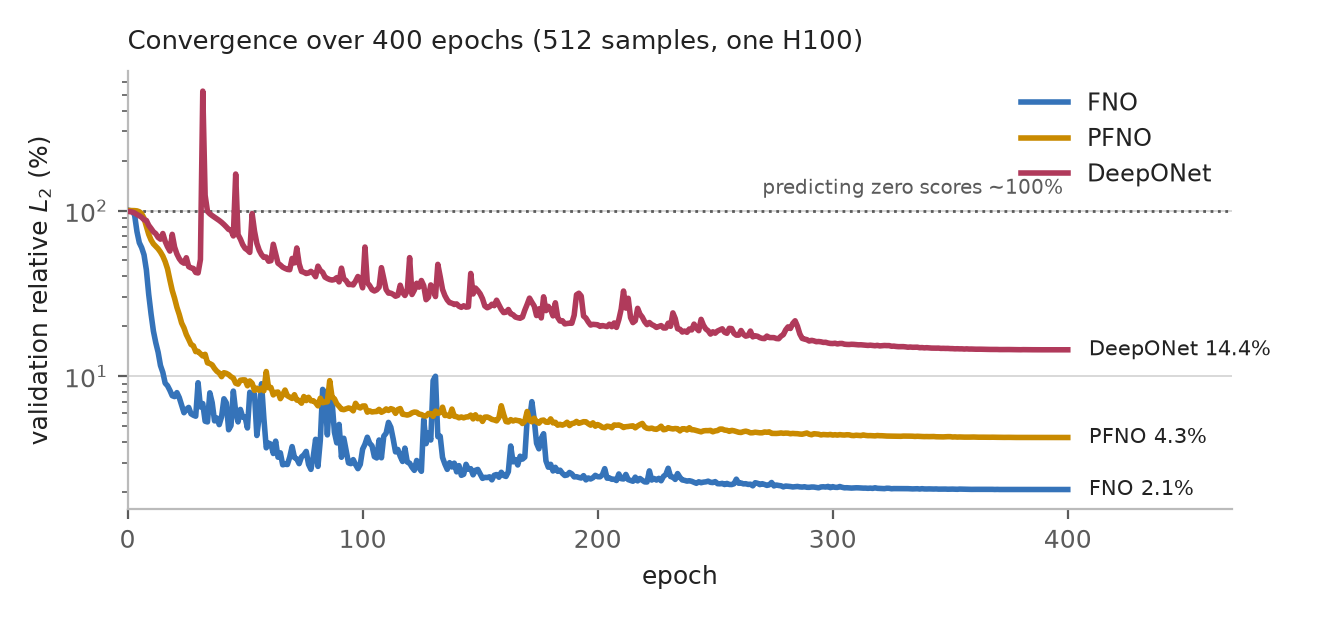
\includegraphics[width=\textwidth]{figures/fig_training_curves.png}
\caption{Convergence of the three operators. All three begin at $\approx100\%$
--- the score of predicting zero --- and the dotted line marks that level. FNO's
visible oscillation is the one-cycle schedule at high learning rate; the best
checkpoint by validation MSE is retained, not the final state.}
\end{figure}

\begin{figure}[htbp]
\centering
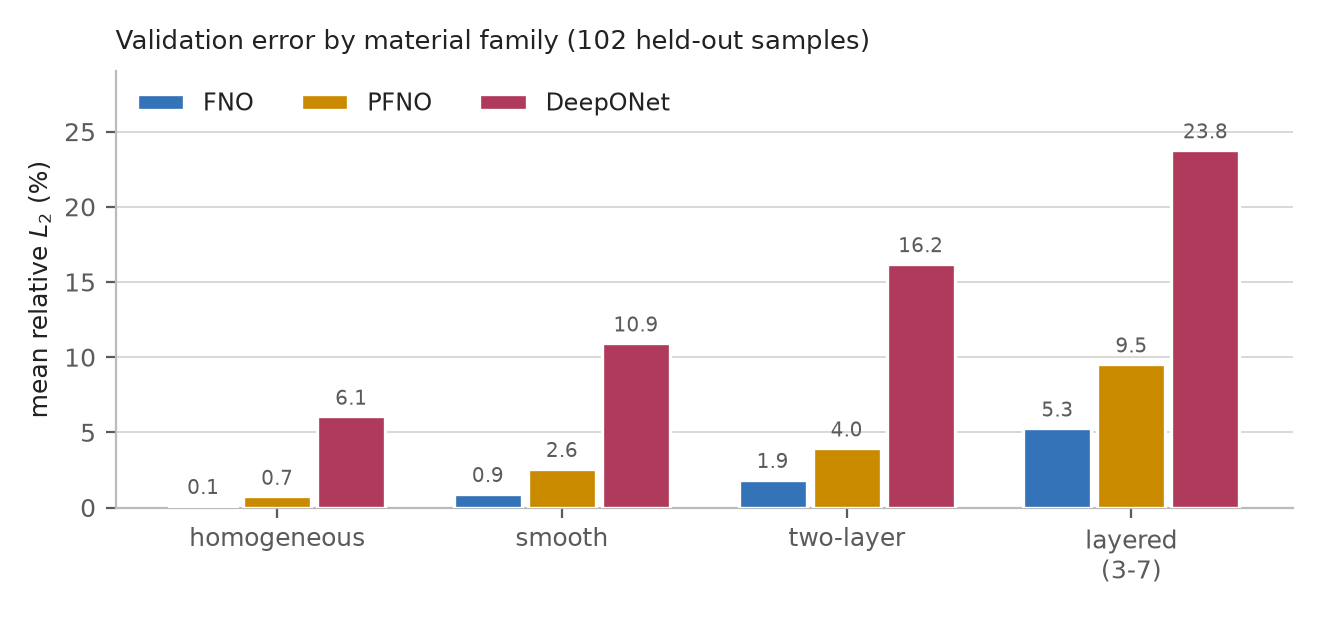
\includegraphics[width=\textwidth]{figures/fig_error_by_material.png}
\caption{Validation error by material family. The ordering is identical for all
three models and matches physical intuition: error grows with the number of
interfaces, since each interface adds a reflected and a transmitted wave the
operator must place correctly.}
\end{figure}

\begin{center}
\small
\begin{tabular}{lrrrr}
\toprule
\textbf{Family} & \textbf{n} & \textbf{FNO} & \textbf{DeepONet} & \textbf{PFNO}\\
\midrule
homogeneous     & 21  & $0.13\%$ & $6.07\%$  & $0.74\%$\\
smooth          & 30  & $0.93\%$ & $10.94\%$ & $2.59\%$\\
two-layer       & 26  & $1.86\%$ & $16.22\%$ & $3.96\%$\\
layered (3--7)  & 25  & $5.28\%$ & $23.78\%$ & $9.55\%$\\
\midrule
\textbf{all}    & \textbf{102} & $\mathbf{2.07\%}$ & $\mathbf{14.43\%}$ & $\mathbf{4.26\%}$\\
\bottomrule
\end{tabular}
\end{center}

Homogeneous media --- a straight V in space--time with no reflections --- are
reproduced nearly exactly. The model ranking (FNO $<$ PFNO $<$ DeepONet) holds
in every family and is what the architectures predict: FNO sees the joint
$(x,t)$ spectrum; PFNO factorizes by temporal frequency and solves each bin with
an independent 1D operator, losing the joint structure; DeepONet compresses the
whole material dependence through a rank-$p$ separable expansion.

%==============================================================
\section{The forced arm: a source term, and its IC/BC residuals}
\label{sec:forced}

Everything above is driven purely by an initial pulse, with no forcing. This
section adds a second, independent arm in which the wave is driven by a source
term instead, and reports how well each model's output respects the initial and
boundary conditions. The unforced arm is unchanged; the two run side by side.

\subsection{Equation and source design}

\begin{equation}
\rho(x)\,u_{tt} \;=\; \frac{\partial}{\partial x}\!\left[E(x)u_x\right]
\;+\; \underbrace{s(x)\,w(t)}_{\text{source}},
\qquad x\in[-1,1],\ t\in[0,2]
\end{equation}

The source is separable, so two input channels carry it exactly:

\begin{itemize}[leftmargin=*,itemsep=2pt]
\item $s(x)=\exp\!\left(-((x-x_s)/w_s)^2\right)$, a narrow Gaussian standing in
for a point source, $w_s=0.04$, position $x_s\sim U(-0.5,0.5)$.
\item $w(t)$ a Ricker wavelet, peak frequency $f\sim U(3,6)$, shifted by
$t_0=1.2/f$ so that $w(0)\approx-1.8\times10^{-5}$ and the start is quiescent to
numerical precision.
\end{itemize}

\noindent The initial conditions become \textbf{quiescent}, $u(x,0)=0$ and
$u_t(x,0)=0$ --- verified exactly zero in the generated data. Boundaries remain
first-order absorbing (Mur), unchanged from the unforced arm.

\paragraph{Why the window is $t\in[0,2]$.} At $t_{\max}=1$ the waves only just
reach the boundary: $99\%$ of the field energy is still inside the domain at the
final step, so the absorbing condition is barely exercised and a boundary
residual would measure almost nothing. Extending to $t_{\max}=2$ lets the waves
fully exit --- $99.8\%$ of the energy has left by the final step --- which is
what makes a BC residual meaningful. The grid is $64\times80$; at
$f\le6$ that is $6.6$--$13$ samples per wavelet period.

\subsection{This is a substantially harder problem}

In the unforced arm only $E(x)$ varied between samples: $\rho\equiv1$, the
initial pulse was fixed, and $x,t$ are fixed meshes. The forced arm has
\textbf{three} varying inputs:

\begin{center}
\small
\begin{tabular}{lrr}
\toprule
\textbf{Channel} & \textbf{Unforced arm} & \textbf{Forced arm}\\
\midrule
$E(x)$              & varies & varies\\
$\rho(x)$           & constant & constant\\
source / IC profile & constant & \textbf{varies} ($x_s$)\\
temporal signature  & --- & \textbf{varies} ($f$)\\
$x$, $t$            & fixed meshes & fixed meshes\\
\bottomrule
\end{tabular}
\end{center}

\noindent The results below should be read against that: the errors are much
larger than the unforced arm's, and the two arms are \emph{not} directly
comparable (different grid, time window, and physics).

\begin{center}
\small
\begin{tabular}{lrrrr}
\toprule
\textbf{Model} & \textbf{Parameters} & \textbf{Train time} & \textbf{Forced rel $L_2$} & \textbf{(Unforced)}\\
\midrule
FNO      & 7{,}387{,}345 & 109\,s  & $\mathbf{17.13\%}$ & $2.07\%$\\
PFNO     & 1{,}524{,}298 & 1273\,s & $\mathbf{31.89\%}$ & $4.26\%$\\
DeepONet &   929{,}281   & 40\,s   & $\mathbf{91.82\%}$ & $14.43\%$\\
\bottomrule
\end{tabular}
\end{center}

\begin{figure}[htbp]
\centering
\makebox[\textwidth][c]{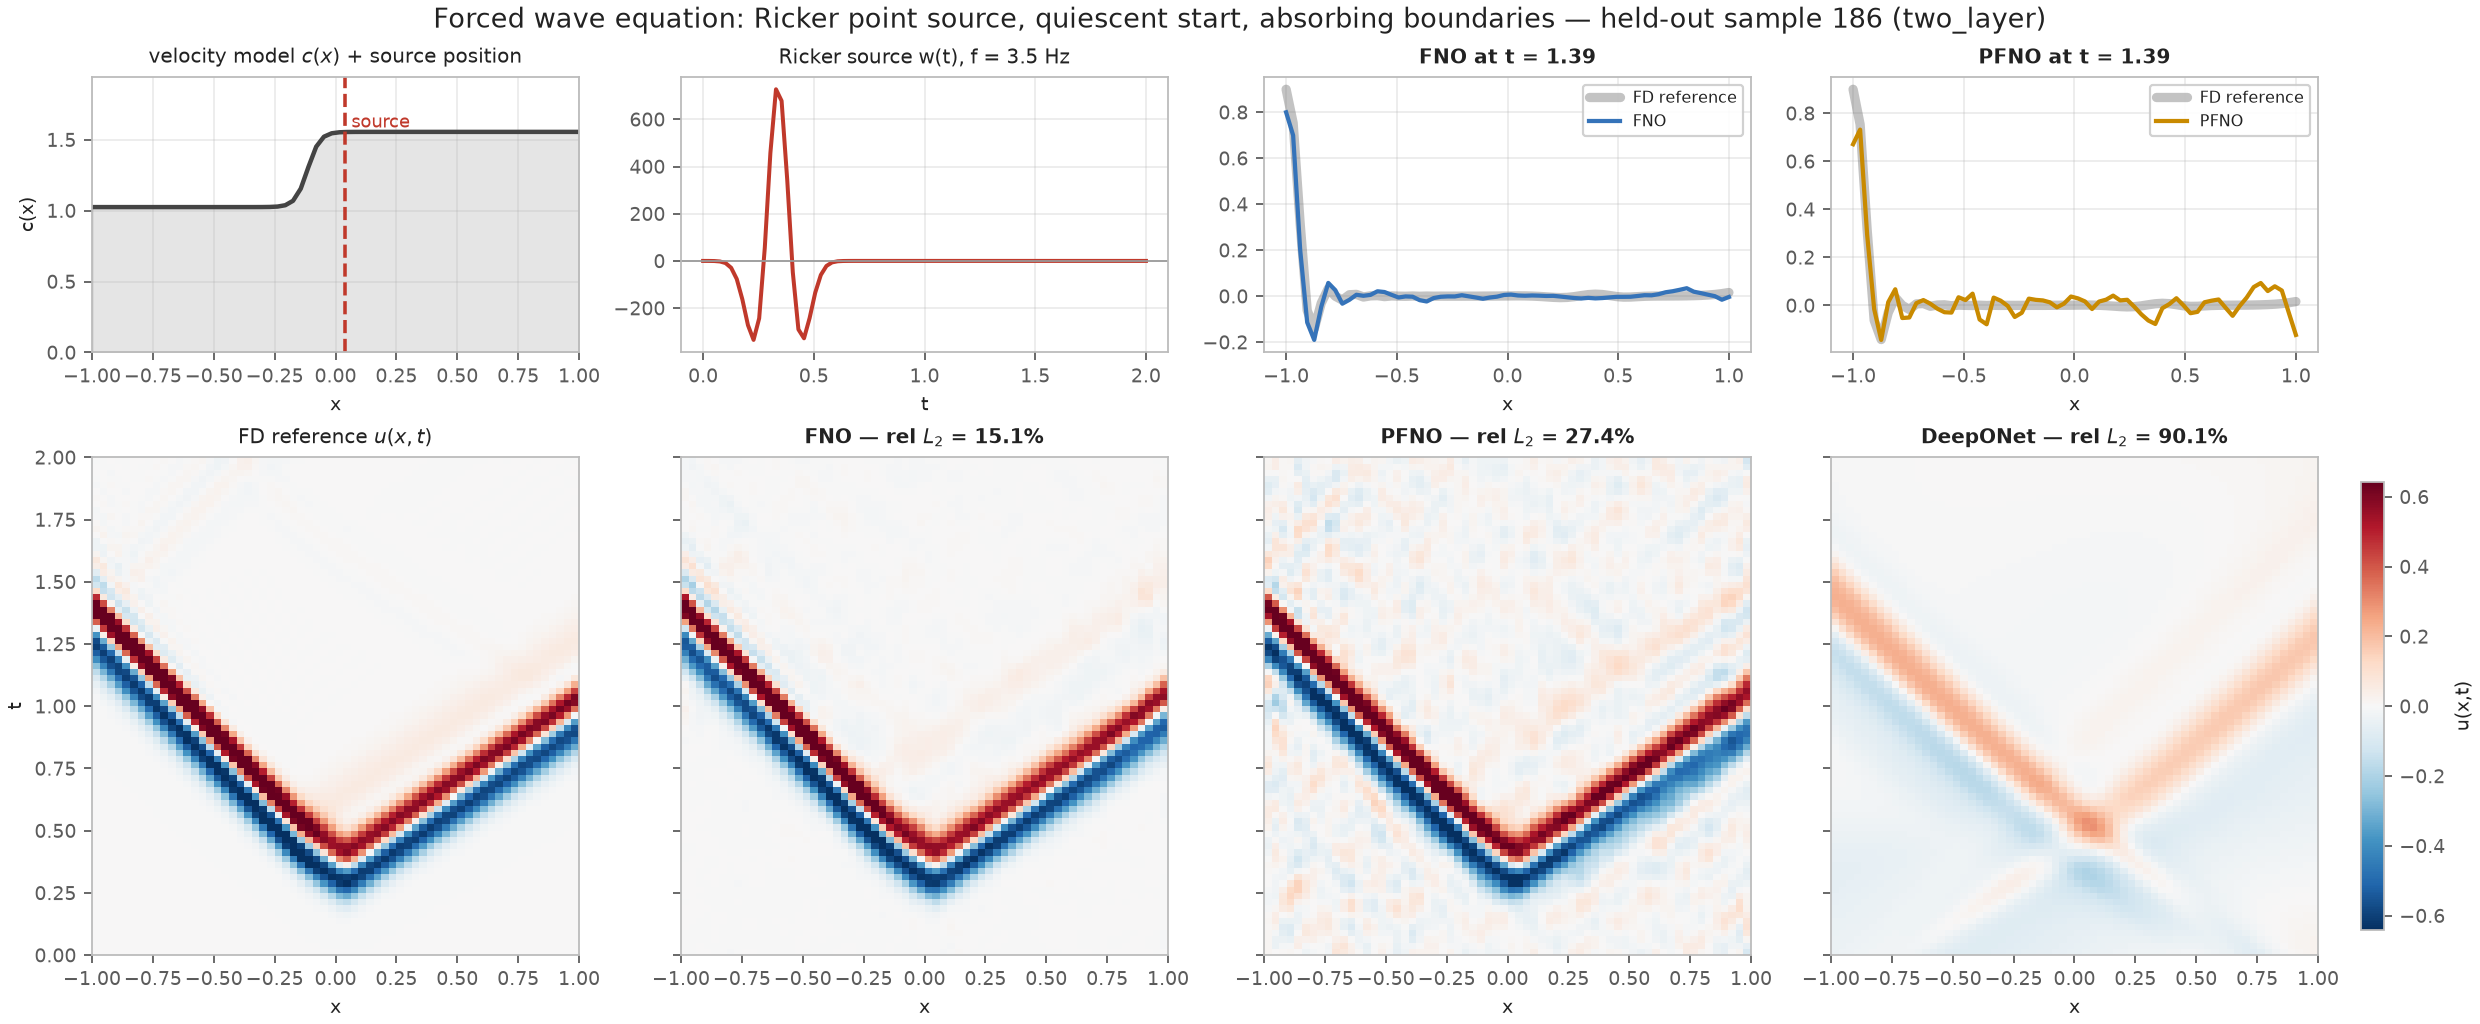
\includegraphics[width=1.18\textwidth]{figures/fig_source_arm.png}}
\caption{Forced arm, a two-layer sample. The source position (dashed red) and
the Ricker wavelet are now inputs. FNO tracks the reference; PFNO reproduces the
arrival but fills the quiet region with speckle; DeepONet produces a smeared
blob where the reference has sharp arrivals.}
\end{figure}

\subsection{Definitions of the residuals}

These are \textbf{diagnostics, not training objectives} --- the loss is still
plain supervised MSE, with no physics term. They answer a question the field
error cannot: does the output respect the conditions it was supposed to inherit?

\paragraph{Initial-condition residuals.} With a quiescent start the targets are
zero, so the residuals are the predicted values themselves:
\begin{equation}
R_{\text{IC}}^{u}=\sqrt{\tfrac1{n_x}\textstyle\sum_i \hat u(x_i,0)^2},
\qquad
R_{\text{IC}}^{u_t}=\sqrt{\tfrac1{n_x}\textstyle\sum_i \hat u_t(x_i,0)^2}.
\end{equation}

\paragraph{Boundary-condition residuals.} The absorbing conditions should
annihilate an outgoing wave:
\begin{equation}
r_L(t)=\hat u_t(-1,t)-c(-1)\,\hat u_x(-1,t),
\qquad
r_R(t)=\hat u_t(+1,t)+c(+1)\,\hat u_x(+1,t),
\end{equation}
reported as an absolute RMS over $t$ and as a scale-free relative version
\begin{equation}
\text{BC}_{\text{rel}}=\frac{\mathrm{RMS}_t(r)}
{\mathrm{RMS}_t(\hat u_t)+\mathrm{RMS}_t(c\,\hat u_x)} .
\end{equation}
All derivatives use second-order finite differences on the output grid
(one-sided at edges).

\paragraph{The reference floor is essential.} The finite-difference solution
satisfies these conditions only to discretisation accuracy on the coarse output
grid --- first-order Mur, plus interpolation from the solver's internal time
step. Its own residual is therefore the achievable floor, and every model number
below is meaningless without it. The metric was validated on two controls: a
standing wave, which violates the outgoing condition maximally, scores
$\text{BC}_{\text{rel}}=1.0000$ exactly; and an all-zero field, which satisfies
both conditions trivially, scores $0$.

\subsection{Results}

\begin{center}
\small
\begin{tabular}{lrrrr}
\toprule
& \textbf{IC displacement} & \textbf{IC velocity} & \textbf{BC absolute} & \textbf{BC relative}\\
\midrule
\textbf{FD reference} & $0$ & $3.9\times10^{-4}$ & $0.886$ & $0.126$\\
\midrule
FNO      & $4.0\times10^{-3}$ & $0.183$ & $1.500$ & $0.249$\\
PFNO     & $3.2\times10^{-2}$ & $1.185$ & $3.691$ & $0.515$\\
DeepONet & $3.3\times10^{-2}$ & $0.269$ & $0.123$ & $\mathbf{0.144}$\\
\bottomrule
\end{tabular}
\end{center}

\subsection{A low boundary residual is not evidence of good physics}

DeepONet reports the \emph{best} boundary score --- $0.144$ relative, and an
absolute residual of $0.123$, seven times \emph{smaller} than the reference's
own $0.886$. It is also by far the worst model, at $91.8\%$ field error.

This is not a contradiction; it is the failure mode the all-zero control
predicted. Decomposing the two terms that are supposed to cancel at the left
boundary, averaged over the validation set:

\begin{center}
\small
\begin{tabular}{lrrr}
\toprule
& \textbf{RMS}\,$u_t$ & \textbf{RMS}\,$c\,u_x$ & \textbf{RMS residual}\\
\midrule
FD reference & $3.285$ & $4.051$ & $0.902$\\
FNO          & $2.817$ & $3.790$ & $1.524$\\
PFNO         & $2.793$ & $4.509$ & $3.603$\\
DeepONet     & $\mathbf{0.561}$ & $\mathbf{0.583}$ & $0.127$\\
\bottomrule
\end{tabular}
\end{center}

\noindent DeepONet's boundary terms are about six times smaller than the
reference's, and its whole-field RMS is $0.41\times$ the reference's. There is
barely a wave arriving at its boundary at all, so it satisfies the radiation
condition by having nothing to radiate. \textbf{IC and BC residuals are
therefore not a standalone quality measure} --- they are only interpretable
alongside the field error.

Among the models that do produce a wave of the right amplitude, the residuals
rank as the field error does: FNO at roughly twice the reference floor, PFNO at
about four times.

\begin{figure}[htbp]
\centering
\makebox[\textwidth][c]{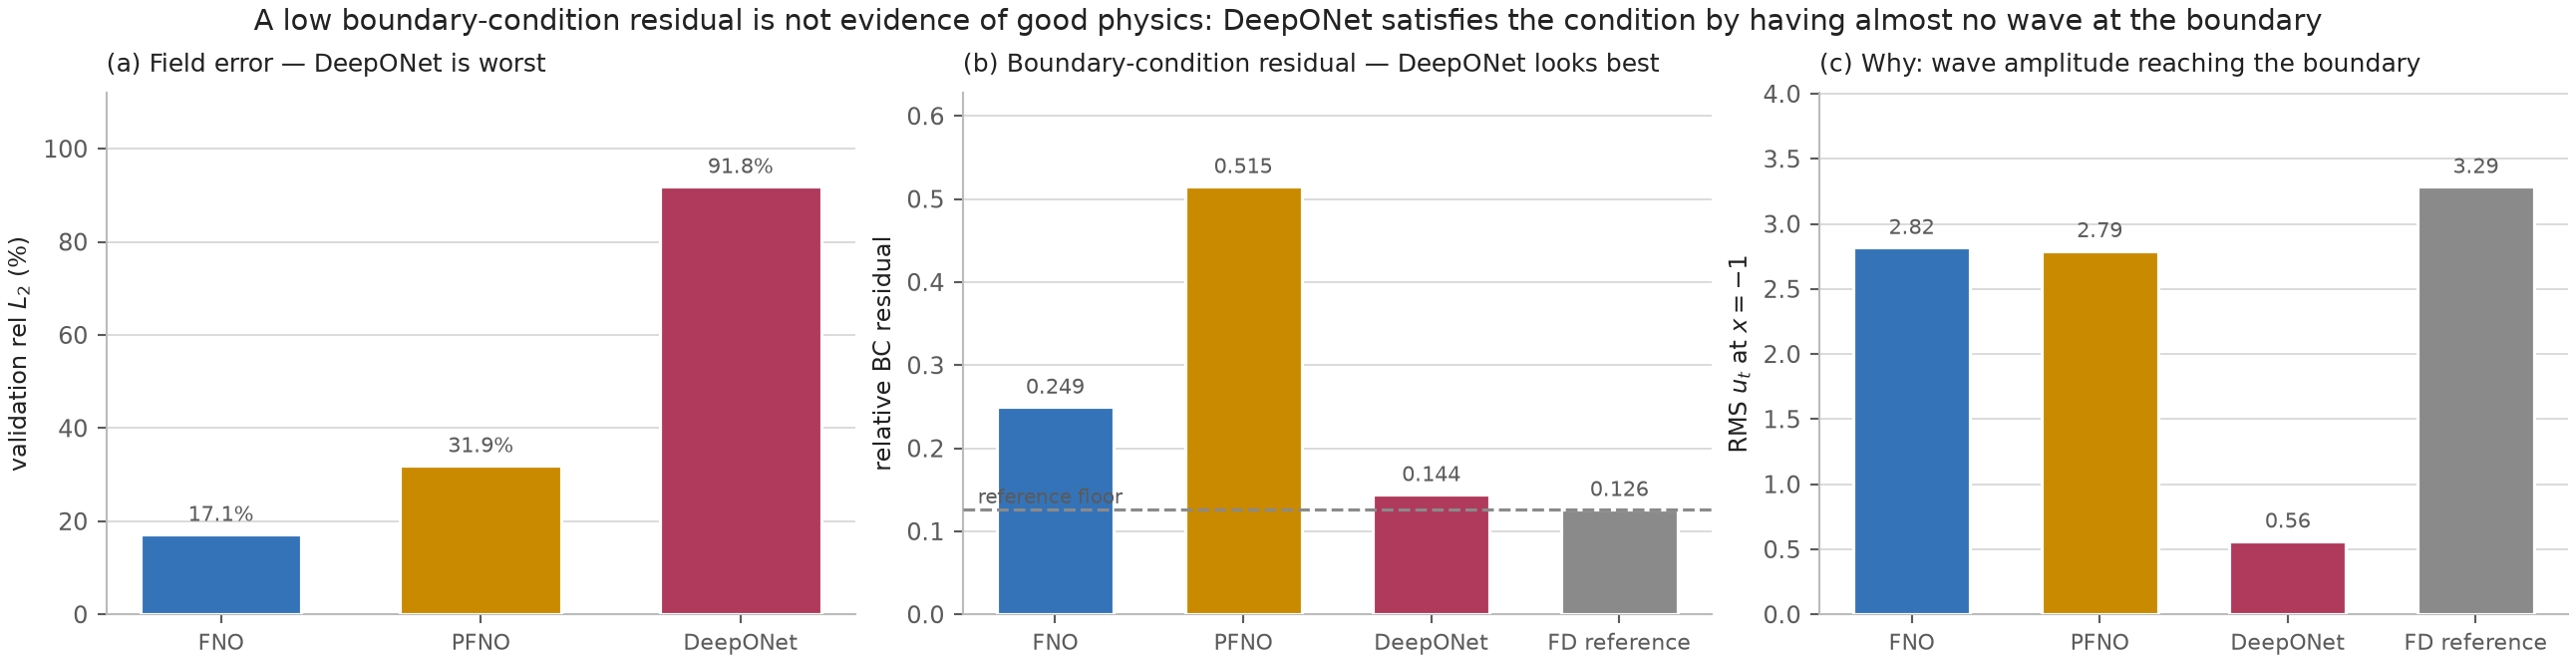
\includegraphics[width=1.16\textwidth]{figures/fig_ic_bc_residuals.png}}
\caption{The same three models, three ways. DeepONet is worst on field error
(a) yet best on boundary residual (b); panel (c) is the explanation --- the wave
amplitude reaching its boundary is a sixth of the reference's.}
\end{figure}

\subsection{PFNO's initial-velocity residual}

One result is disproportionate rather than merely ordered. PFNO's IC velocity
residual is $1.185$, six times FNO's $0.183$, although its field error is only
$1.9\times$ FNO's.

The cause is structural. PFNO assembles the field from $n_t/2+1=41$ independent
temporal-frequency branches. Enforcing $u_t(x,0)=0$ requires the phases of all
41 bins to agree precisely at $t=0$; small independent per-bin errors barely
perturb the field but accumulate directly in its time derivative. The speckle
filling the quiet region of PFNO's panel in the figure above is the same effect
seen in the field.

%==============================================================
\section{Making IC and BC actual training losses}
\label{sec:pinn}

Section~\ref{sec:forced} treats the residuals purely as diagnostics: the loss is
supervised MSE and nothing about the physics reaches the gradients. This section
adds them to the objective,
\begin{equation}
\mathcal{L} \;=\; \underbrace{\mathrm{MSE}(\hat y,\,y)}_{\text{data}}
\;+\;\lambda\Bigl(\mathcal{L}^{u}_{\text{IC}}+\mathcal{L}^{u_t}_{\text{IC}}
+\mathcal{L}_{\text{BC}}\Bigr),
\end{equation}
which is the PINN-style treatment already used on the coordinate-network side of
this repository (\texttt{src/losses/wave\_loss.py}).

\paragraph{Implementation.} \texttt{physics\_metrics.py} is numpy and cannot
backpropagate, so the same quantities are reimplemented in torch in
\texttt{physics\_losses\_torch.py}. The two agree to $\sim\!10^{-8}$, float32
precision --- verified before any of the results below were trusted. Each term is
divided by a fixed scale precomputed from the training targets (RMS of $u$, of
$u_t$, and of the boundary terms), so all three land in a comparable range and a
single $\lambda$ balances them against the data term. The scales are constants,
not batch statistics: a data-dependent denominator inside a loss makes gradients
noisy. Setting \texttt{-{}-lambda-physics 0} reproduces the supervised run
exactly.

\subsection{Weight sweep}

\begin{center}
\small
\begin{tabular}{rrrrr}
\toprule
$\lambda$ & \textbf{Field error} & \textbf{IC displacement} & \textbf{IC velocity} & \textbf{BC relative}\\
\midrule
$0$ (baseline) & $17.13\%$ & $4.03\times10^{-3}$ & $0.1835$ & $0.2494$\\
$0.003$        & $17.02\%$ & $3.47\times10^{-3}$ & $0.1507$ & $0.2380$\\
$0.03$         & $16.92\%$ & $2.04\times10^{-3}$ & $0.0884$ & $0.1928$\\
$0.3$          & $15.89\%$ & $1.36\times10^{-3}$ & $0.0461$ & $0.1205$\\
$1.0$          & $14.84\%$ & $5.15\times10^{-4}$ & $0.0171$ & $0.0657$\\
$3.0$          & $14.20\%$ & $7.56\times10^{-4}$ & $0.0151$ & $0.0426$\\
$10.0$         & $\mathbf{12.70\%}$ & $\mathbf{1.95\times10^{-4}}$ & $\mathbf{0.0058}$ & $\mathbf{0.0291}$\\
\bottomrule
\end{tabular}
\end{center}

\noindent FNO, 500 epochs per point. Every metric improves monotonically and
\textbf{no trade-off appears} --- not even at $\lambda=10$, where the physics
terms dominate the objective. Field error falls $26\%$ in relative terms and the
initial-velocity residual improves $32\times$.

That is unusual enough to be worth suspecting, so the collapse check from
Section~\ref{sec:forced} was repeated: at $\lambda=1$ the field RMS is
$0.982\times$ the reference, against $0.969\times$ for the supervised baseline.
The model is \emph{more} faithful in amplitude, not less, so the gain is real
rather than the degenerate solution reappearing. The likely reason is
regularisation: with $410$ training samples on a hard problem, the constraints
supply true information about the solution that the data alone does not pin down.

\begin{figure}[htbp]
\centering
\makebox[\textwidth][c]{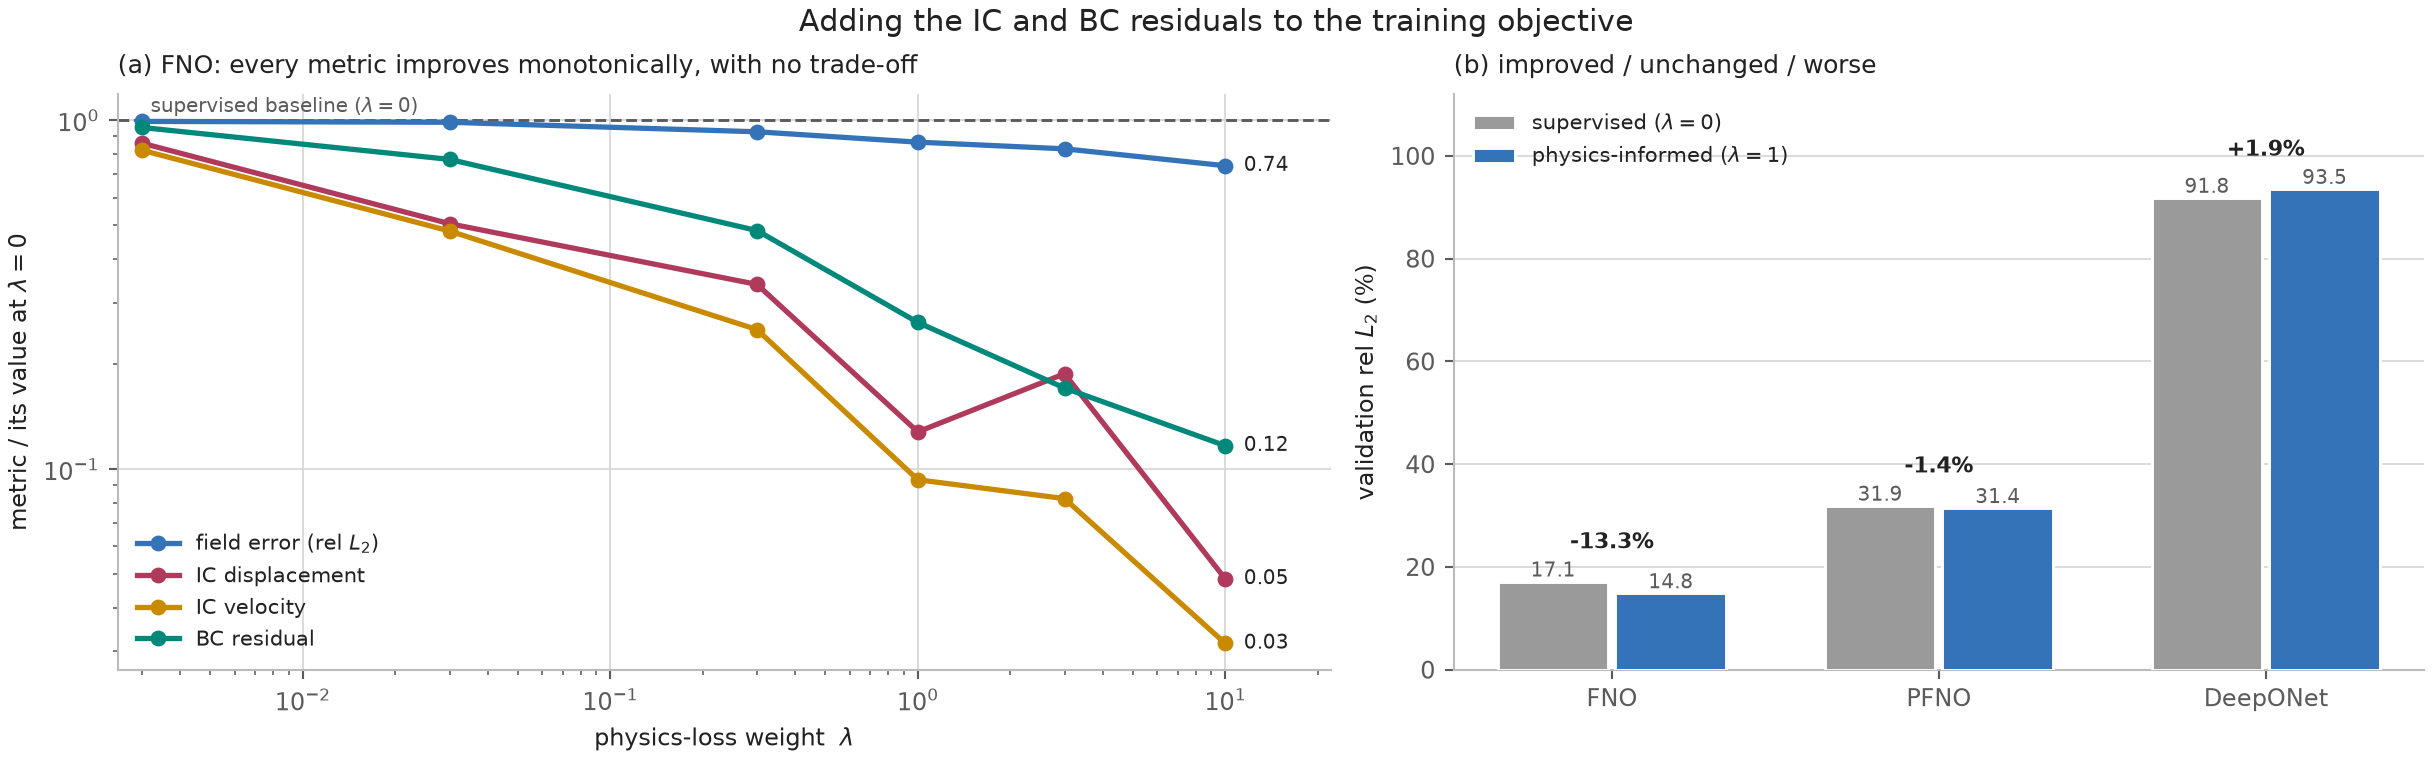
\includegraphics[width=1.16\textwidth]{figures/fig_physics_informed.png}}
\caption{(a) Every metric, normalised by its own supervised baseline; below the
dashed line is an improvement. (b) The same weight applied to all three
architectures gives three different outcomes.}
\end{figure}

\subsection{Three architectures, three outcomes}

All three trained at $\lambda=1$ --- a round value inside the beneficial regime,
chosen over the sweep's best because PFNO's raw physics loss is about six times
FNO's, so the same weight bites considerably harder there.

\begin{center}
\small
\begin{tabular}{lrrrrrr}
\toprule
& \multicolumn{2}{c}{\textbf{Field error}} & \multicolumn{2}{c}{\textbf{IC velocity}} & \multicolumn{2}{c}{\textbf{BC relative}}\\
\cmidrule(lr){2-3}\cmidrule(lr){4-5}\cmidrule(lr){6-7}
& $\lambda=0$ & $\lambda=1$ & $\lambda=0$ & $\lambda=1$ & $\lambda=0$ & $\lambda=1$\\
\midrule
FNO      & $17.13\%$ & $\mathbf{14.84\%}$ & $0.183$ & $\mathbf{0.017}$ & $0.249$ & $\mathbf{0.066}$\\
PFNO     & $31.89\%$ & $31.43\%$          & $1.185$ & $0.833$          & $0.515$ & $0.386$\\
DeepONet & $91.82\%$ & $93.55\%$          & $0.269$ & $0.148$          & $0.144$ & $0.144$\\
\bottomrule
\end{tabular}
\end{center}

\paragraph{FNO --- improved on every axis.} Its relative boundary residual,
$0.066$, is now half the finite-difference reference's own $0.126$. That is not
``better than the truth'': the reference's residual comes from its first-order
Mur discretisation, and the network is under no obligation to reproduce that
particular error while still sitting $15\%$ away in $L_2$.

\paragraph{PFNO --- essentially unchanged.} This was the architecture predicted
to benefit most, since its initial-velocity residual was its clearest structural
weakness. It did not: field error moved $31.9\to31.4\%$ and the residual only
$1.185\to0.833$. The prediction was wrong, and the reason is the more
interesting result. PFNO's $41$ frequency branches are independent networks with
no mechanism to coordinate phase; a gradient on the assembled field cannot
easily repair a coordination failure distributed across $41$ separate
sub-networks. The defect is architectural, not an optimisation shortfall.

\paragraph{DeepONet --- worse.} Field error rose $91.8\to93.6\%$ and the field
amplitude fell further, $0.409\to0.374$ of the reference. This is the sharpest
lesson of the section. Zero satisfies every one of these homogeneous constraints
\emph{exactly}, so for a model that already cannot fit the data the physics terms
are a gradient pointing \textbf{toward} the trivial solution. Physics-informed
training reinforces collapse when the model lacks the capacity to fit the data;
the constraints only help once a model is good enough that satisfying them is
non-trivial.

%==============================================================
\section{Real velocity models: Marmousi, Overthrust, Salt}\label{sec:real}

Everything above draws $E(x)$ from a synthetic sampler --- tanh steps and sums
of sinusoids. This section replaces that sampler with 1D depth columns taken
from three published velocity models, keeping the problem, the solver, the
architectures and the training schedule identical.

\textbf{What is real here, and what is not.} The \emph{material} is real, in the
sense that these are the models the exploration-geophysics community uses as
ground-truth benchmarks. They are not field measurements: Marmousi and
Overthrust are both synthetic constructions designed to be geologically
realistic. Well logs would be genuinely measured $V_p(z)$; these are a step
short of that but far beyond tanh profiles. The \emph{wave field} is still
FD-simulated in every case, because no measured full-field $u(x,t)$ exists for
this geometry --- the target has to be computed either way.

\begin{center}
\small
\begin{tabular}{llllll}
\toprule
\textbf{Model} & \textbf{Geometry} & \textbf{Spacing} & \textbf{Density} & \textbf{$V_p$ range} & \textbf{Source}\\
\midrule
\texttt{marmousi}   & $2301\times739$          & 4\,m  & measured        & 1532--5500\,m/s & geoazur WIND\\
\texttt{overthrust} & $801\times801\times161$  & 25\,m & none ($\rho=1$) & 2182--6000\,m/s & SEG/EAGE\\
\texttt{salt}       & $676\times676\times180$  & 20\,m & none ($\rho=1$) & 1500--4482\,m/s & SEG/EAGE\\
\bottomrule
\end{tabular}
\end{center}

Water caps and constant basements are trimmed. Each sample takes a random
contiguous depth window from a random trace, reduced onto the 64-point grid by
\textbf{Backus averaging} --- arithmetic mean of $\rho$, harmonic mean of the
modulus $M=\rho V_p^2$, the correct long-wavelength effective medium for
normal-incidence 1D propagation. Point-sampling a 739-sample column down to 64
would alias the interfaces into noise: $3.2\%$ of Marmousi's cells jump by more
than 200\,m/s, with a maximum of 1530\,m/s in a single 4\,m cell.

Wave speed is preserved exactly by the nondimensionalisation. Dividing by fixed
per-model reference values (the medians $V_p^{\mathrm{ref}}$,
$\rho^{\mathrm{ref}}$) gives $\tilde c=\sqrt{\tilde E/\tilde\rho}=V_p/V_p^{\mathrm{ref}}$,
so genuine sample-to-sample speed variation survives instead of being normalised
away.

\subsection{Three methodological changes the real data forces}

\textbf{Density varies (Marmousi only).} Marmousi ships a density model, so
channel 1 is no longer all ones. Overthrust and Salt ship velocity only and get
$\rho=1$ like the synthetic arm. Gardner's relation could synthesise a density,
but it is an empirical fit --- it would add fiction while claiming realism.

\textbf{The train/validation split must be spatial.} Neighbouring Marmousi
traces are 4\,m apart and differ by a mean $|\Delta V_p|$ of 6\,m/s --- $0.2\%$
of the mean. Even 20 traces apart the difference is only $3.7\%$. Drawing 512
samples at random from 2301 traces puts near-duplicates of training profiles
into validation, and the resulting ``generalisation'' error is really an
interpolation error. Validation instead takes four contiguous trace blocks
spread across the model, with 320\,m buffers discarded on each side; the
realised minimum train-to-validation separation is 328\,m (Marmousi), 400\,m
(Overthrust), 420\,m (Salt). The split ships inside the dataset as a
\texttt{split} array, and \texttt{train\_operators.py} honours it when present,
falling back to its random split otherwise.

\textbf{The FD target has to be grid-converged.} This turned out to matter far
more than expected, and it applies to the synthetic arm too.

\subsection{The target was not converged}\label{sec:refine}

The original datasets solve the FD reference on the same 64-point grid as the
output. Measured against a \texttt{refine=32} reference:

\begin{center}
\small
\begin{tabular}{lrrr}
\toprule
\textbf{refine} & \textbf{FD grid} & \textbf{\relL{} vs converged} & \textbf{Cost / 512}\\
\midrule
1            & 64            & $13.35\%$            & 1.8\,s\\
2            & 127           & $3.87\%$             & 2.9\,s\\
4            & 253           & $1.14\%$             & 8.9\,s\\
\textbf{8}   & \textbf{505}  & $\mathbf{0.32\%}$    & \textbf{22\,s}\\
16           & 1009          & $0.08\%$             & 41\,s\\
\bottomrule
\end{tabular}
\end{center}

Regenerating the synthetic dataset with \textbf{identical materials} (same seed,
same sampler --- the \texttt{inputs} arrays are bit-identical) and only a
converged target moves the targets by $\mathbf{9.72\%}$ on average, and by
$7.91\%$ even on \texttt{homogeneous} samples, which contain no interfaces at
all. That part is not interface error: it is numerical dispersion of the initial
pulse itself, whose width $\sigma_g=0.1$ spans only about three cells at 64
points.

What happens when the models are retrained against the corrected target is the
interesting part:

\begin{center}
\small
\begin{tabular}{lrr}
\toprule
\textbf{Model} & \textbf{vs \texttt{refine=1}} & \textbf{vs \texttt{refine=8}}\\
\midrule
FNO      & $2.07\%$  & $\mathbf{1.96\%}$\\
PFNO     & $4.26\%$  & $\mathbf{4.03\%}$\\
DeepONet & $14.43\%$ & $\mathbf{24.57\%}$\\
\bottomrule
\end{tabular}
\end{center}

FNO and PFNO are essentially unchanged. The discretisation error is a
deterministic function of the material, not noise, so a model with enough
capacity simply learns whichever target it is given and scores the same against
it. The published $2.07\%$ was therefore never \emph{inflated} --- but it should
be read as ``$2\%$ away from the 64-point FD solution'', not ``$2\%$ away from
the wave''.

DeepONet is the exception: it nearly doubles. The \texttt{refine=1} target is
smoother --- dispersion smears the pulse --- and a rank-$p$ separable expansion
$u\approx\sum_p b_p(E)\,\tau_p(x,t)$ represents smooth fields much more cheaply
than sharp ones. The under-resolved target was flattering it. This is worth
stating plainly: one of the three architectures had its headline number
materially improved by a numerical artefact, and the effect was invisible until
the target was fixed.

\subsection{Results}

512 samples per arm, 400 epochs, AdamW (lr $3\times10^{-3}$, weight decay
$10^{-4}$), batch 16, NVIDIA H100 NVL. All four arms use \texttt{refine=8}
targets; the three real arms use disjoint trace-block splits. Parameter counts
are identical across arms (FNO 7{,}387{,}297; PFNO 1{,}225{,}290; DeepONet
888{,}321).

\begin{figure}[htbp]
\centering
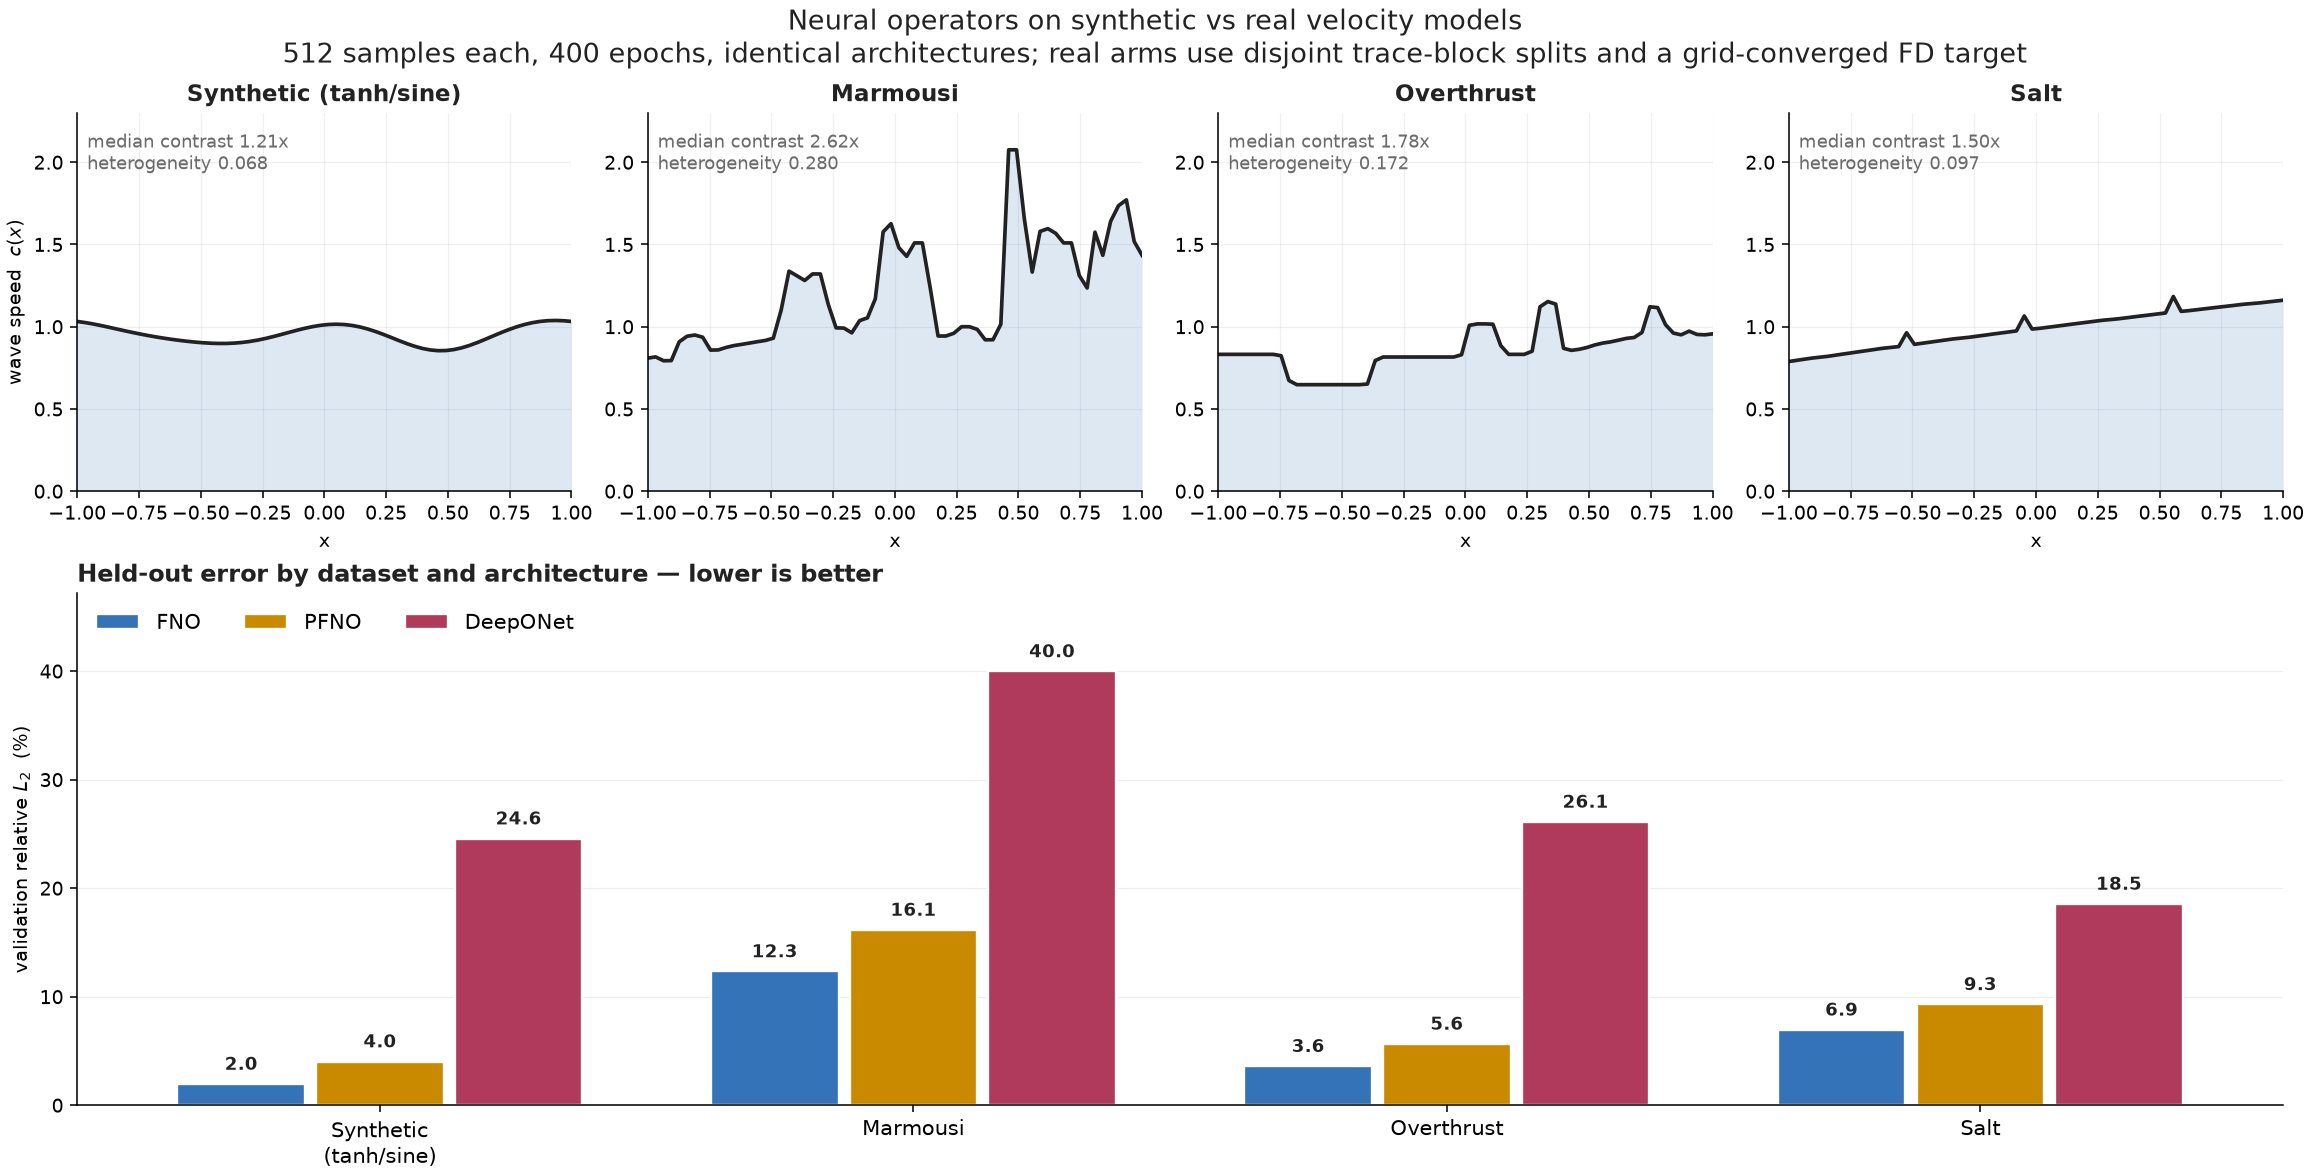
\includegraphics[width=\textwidth]{figures/real_models_comparison.png}
\caption{Held-out error by dataset and architecture. Top row: a
median-contrast velocity profile from each arm, with its heterogeneity (median
within-sample standard deviation of $c(x)$). The architectural ranking
FNO $<$ PFNO $<$ DeepONet holds on every dataset, but the margins compress as
the material stops being smooth.}
\end{figure}

\begin{center}
\small
\begin{tabular}{lrrrrr}
\toprule
\textbf{Arm} & \textbf{Heterogeneity} & \textbf{Median contrast} & \textbf{FNO} & \textbf{PFNO} & \textbf{DeepONet}\\
\midrule
synthetic (tanh/sine) & 0.068 & $1.21\times$ & $\mathbf{1.96\%}$  & $\mathbf{4.03\%}$  & $\mathbf{24.57\%}$\\
Overthrust            & 0.172 & $1.78\times$ & $\mathbf{3.59\%}$  & $\mathbf{5.65\%}$  & $\mathbf{26.11\%}$\\
Salt                  & 0.097 & $1.50\times$ & $\mathbf{6.95\%}$  & $\mathbf{9.30\%}$  & $\mathbf{18.55\%}$\\
Marmousi              & 0.280 & $2.62\times$ & $\mathbf{12.33\%}$ & $\mathbf{16.15\%}$ & $\mathbf{39.97\%}$\\
\bottomrule
\end{tabular}
\end{center}

\textbf{The architectural ranking survives.} FNO $<$ PFNO $<$ DeepONet on every
arm, without exception. The conclusion drawn from synthetic data holds on real
geology, which is the main thing this section was run to check.

\textbf{The margins compress.} On synthetic data FNO beats PFNO by $2.1\times$;
on Marmousi by $1.3\times$. The gap that separates a joint $(x,t)$ spectral
operator from a per-frequency one narrows once the material stops being smooth
--- both are struggling with the same thing.

\textbf{Difficulty tracks heterogeneity, not contrast.} Marmousi is $4.1\times$
more heterogeneous than the synthetic set and $6\times$ harder for FNO.
Overthrust, with a similar velocity range but much smoother columns, costs only
$1.8\times$.

\subsection{Contrast is a poor difficulty predictor}

Grouping each arm's validation samples into per-model contrast terciles gives a
result that does not generalise:

\begin{center}
\small
\begin{tabular}{lrrr}
\toprule
\textbf{Arm} & \textbf{Low contrast} & \textbf{Moderate} & \textbf{High contrast}\\
\midrule
Marmousi   & $14.96\%$ & $12.16\%$ & $\mathbf{9.87\%}$\\
Overthrust & $5.02\%$  & $3.33\%$  & $\mathbf{2.67\%}$\\
Salt       & $3.49\%$  & $2.88\%$  & $\mathbf{13.26\%}$\\
\bottomrule
\end{tabular}
\end{center}

\noindent(FNO; PFNO and DeepONet show the same shape.)

Marmousi and Overthrust get \emph{easier} as contrast rises. That is not a
normalisation artefact --- across Marmousi's bands $\|\text{target}\|$ rises
only $2\%$ while FNO's absolute $L_2$ error falls $33\%$. The plausible reading
is that strong reflectors produce distinct, high-amplitude coherent arrivals
that are structurally easy to learn, whereas low-contrast windows give weak
diffuse scattering: subtle, low-amplitude deviations from a smooth background.

Salt reverses it completely --- its high-contrast band is $4.6\times$ worse than
its moderate band. The explanation is geological rather than statistical: Salt's
low- and moderate-contrast columns are mostly a smooth sediment velocity
gradient, while the high-contrast columns are exactly the ones that intersect a
salt body, where $V_p$ jumps from ${\sim}2000$ to 4482\,m/s across a sharp,
isolated boundary. A single strong impedance jump is a different and harder
problem than a gradual increase in range.

So $V_p^{\max}/V_p^{\min}$ summarises the wrong thing. What predicts difficulty
is whether the column contains a sharp isolated reflector, not how wide its
velocity range is. The per-model terciles behind the \texttt{kinds} labels are
therefore useful only \emph{within} a model --- Marmousi's high band starts at
$2.96\times$ and Salt's at $1.61\times$; the datasets carry the absolute
\texttt{contrast} array for cross-model work.

\subsection{Animations}\label{sec:realgifs}

Nine GIFs in \texttt{simulations/real/<model>/}, one per contrast band per
model, each the \textbf{median-error} sample of its band. Layout and colour
scale are identical to the synthetic ones (\S\ref{sec:viz}), so they can be read
side by side.

\begin{center}
\small
\begin{tabular}{llrrrr}
\toprule
\textbf{Model} & \textbf{Band} & \textbf{Sample} & \textbf{FNO} & \textbf{PFNO} & \textbf{DeepONet}\\
\midrule
Marmousi   & low      & 412 & $12.74\%$ & $13.49\%$ & $40.55\%$\\
Marmousi   & moderate & 458 & $11.05\%$ & $15.75\%$ & $39.34\%$\\
Marmousi   & high     & 499 & $10.20\%$ & $13.66\%$ & $32.74\%$\\
\midrule
Overthrust & low      & 499 & $4.49\%$  & $6.40\%$  & $28.15\%$\\
Overthrust & moderate & 491 & $2.84\%$  & $4.25\%$  & $21.65\%$\\
Overthrust & high     & 458 & $2.03\%$  & $3.69\%$  & $25.23\%$\\
\midrule
Salt       & low      & 470 & $3.25\%$  & $4.49\%$  & $10.51\%$\\
Salt       & moderate & 419 & $\mathbf{2.70\%}$ & $\mathbf{2.41\%}$ & $8.08\%$\\
Salt       & high     & 458 & $10.69\%$ & $18.94\%$ & $45.03\%$\\
\bottomrule
\end{tabular}
\end{center}

The two Salt entries are the pair worth watching. Sample 419 is among the
easiest in the whole study --- a smooth sediment gradient, and the only
animation anywhere in which \textbf{PFNO beats FNO} ($2.41\%$ against $2.70\%$;
one sample, so noise rather than a real reversal). Sample 458 is the same model
at $4\times$ the error, because that column crosses a salt body: the reflection
off the boundary is visible in the FD panel, and all three predictions blur it.

Note that the sample ids repeat across models (458 appears three times). They
are indices into each arm's own validation set, not a shared identifier.

\subsection{Reproducing}

\begin{lstlisting}
# Fetch models into operator_data/raw/ (URLs in wave/operator_sim/README.md)
python wave/operator_sim/generate_dataset_real.py --model marmousi \
    --num-samples 512 --seed 42 \
    --out operator_data/wave_operator_marmousi_n512_nx64_nt64_t1_seed42.npz

# Synthetic arm, now with a converged target
python wave/operator_sim/generate_dataset.py --refine 8 --num-samples 512 \
    --seed 42 \
    --out operator_data/wave_operator_fixedic_r8_n512_nx64_nt64_t1_seed42.npz

# Train (GPU). NOTE --don-latent/--don-hidden: the script defaults are
# 192/384, but every result quoted here uses the larger 256/512 pair.
python wave/operator_sim/train_operators.py --data <npz> --epochs 400 \
    --don-latent 256 --don-hidden 512 --outdir out_<arm>
\end{lstlisting}

%==============================================================
\section{Visualization design}\label{sec:viz}

Two defects in the original figure were fixed. Both affected interpretability
independently of model quality.

\paragraph{1. The reference is now shown.} The original compared the three
predictions \emph{against each other only}, reporting a pairwise disagreement
matrix. This is actively misleading when models are undertrained: a near-zero
field looks smooth and plausible, and the disagreement numbers ($110$--$140\%$)
were large without indicating which model, if any, was right. Every panel now
sits against the FD reference, and titles carry the per-sample \relL{}.

\paragraph{2. The colour scale is set from the propagating wave.} The $t=0$
pulse has unit amplitude but immediately splits into two waves of $\approx0.5$
each. Measured across all 512 samples:

\begin{center}
\small
\begin{tabular}{lr}
\toprule
$\max|u|$ over all $t$                & $1.00$\\
$\max|u|$ for $t>0$                   & $0.97$ \quad\textit{(frame 1 still contains the pulse)}\\
98th percentile of $|u|$              & $\mathbf{0.55}$ \quad\textit{(the propagating amplitude)}\\
\bottomrule
\end{tabular}
\end{center}

Scaling \texttt{vmin}/\texttt{vmax} to the global maximum therefore spent half
the colormap on a single frame and pushed everything afterwards into the pale
middle. The scale is now the 98th percentile of $|u|$, computed from the
reference and shared across all four field panels. The initial pulse saturates
for the first few frames, which is the intended trade.

\begin{lstlisting}
# Colour: propagating wave, not the t=0 pulse (~1.8x taller).
amplitude = max(float(np.percentile(np.abs(reference), 98.0)), 1e-6)
# Line plots keep the full range so the initial pulse is not clipped.
line_amplitude = max(float(np.abs(reference).max()),
                     max(float(np.abs(f).max()) for f in wavefields.values()), 1e-6)
\end{lstlisting}

\paragraph{3. The series palette was re-stepped.} The original blue/teal pair
for FNO and DeepONet sat at $\Delta E=14.0$ under normal colour vision, below
the legibility floor --- hard to separate even with full colour vision, and
worse under simulated deuteranopia. The palette is now
\textcolor{fnoblue}{$\blacksquare$~FNO \texttt{\#3573B9}},
\textcolor{donrose}{$\blacksquare$~DeepONet \texttt{\#B03A5B}},
\textcolor{pfnogold}{$\blacksquare$~PFNO \texttt{\#C98A00}},
whose worst adjacent pair is $\Delta E=16.0$ (protanopia) and $22.8$ (normal
vision). Panel titles are set in ink rather than the series colour; identity is
carried by the coloured line in the legend, so no text depends on colour to be
readable.

\medskip\noindent
Smaller choices, for the record: the reference curve is drawn thick and pale
\emph{underneath} the thin coloured prediction, so overlap stays legible and any
deviation reads immediately; the velocity model $c(x)$ is shown so wave
behaviour is explicable from the input; and the rendered samples are the
median-error sample per family rather than the best, so the animations are
representative.

%==============================================================
\section{The code}

Everything lives in \texttt{wave/operator\_sim/}.

\begin{center}
\small
\begin{tabular}{ll}
\toprule
\textbf{File} & \textbf{Role}\\
\midrule
\texttt{generate\_dataset.py}    & FD dataset generation (wraps the repo's sampler and solver)\\
\texttt{operator\_models.py}     & The three architectures, verbatim from the notebook\\
\texttt{train\_operators.py}     & Training loop, evaluation, prediction export\\
\texttt{render\_simulations.py}  & Animation rendering\\
\texttt{README.md}               & Quick-start summary\\
\bottomrule
\end{tabular}
\end{center}

The split between training and rendering is deliberate: training writes
\emph{no} plots, so the GPU host needs no matplotlib. Training exports
predictions to an \texttt{.npz}, and rendering happens wherever matplotlib is
available.

\subsection{Training core}

\begin{lstlisting}
opt = torch.optim.AdamW(model.parameters(), lr=a.lr, weight_decay=a.weight_decay)
sched = torch.optim.lr_scheduler.OneCycleLR(
    opt, max_lr=a.lr, total_steps=a.epochs * len(train_loader), pct_start=0.15)

for epoch in range(1, a.epochs + 1):
    model.train()
    for xb, yb in train_loader:
        xb, yb = xb.to(DEVICE), yb.to(DEVICE)
        opt.zero_grad(set_to_none=True)
        loss = F.mse_loss(model(xb), yb)
        loss.backward(); opt.step(); sched.step()
    vmse, vrel = evaluate(model)
    if vmse < best_val:                       # keep the best, not the last
        best_val = vmse
        best_state = copy.deepcopy(model.state_dict())
\end{lstlisting}

Evaluation de-normalizes before measuring, so the reported error is in physical
units:

\begin{lstlisting}
@torch.no_grad()
def evaluate(model):
    model.eval(); se = 0.0; n = 0; rels = []
    for xb, yb in val_loader:
        xb, yb = xb.to(DEVICE), yb.to(DEVICE)
        pred, tgt = denorm(model(xb)), denorm(yb)
        se += F.mse_loss(pred, tgt, reduction="sum").item(); n += tgt.numel()
        pf, tf = pred.flatten(1), tgt.flatten(1)
        rel = (torch.linalg.vector_norm(pf - tf, dim=1)
               / torch.linalg.vector_norm(tf, dim=1).clamp_min(1e-12))
        rels.extend((100.0 * rel).cpu().tolist())
    return se / n, float(np.mean(rels))
\end{lstlisting}

The run exports \texttt{operator\_wave\bk\_predictions\bk\_v2.npz} containing $x$, $t$,
the validation ids and kinds, the $E$ and $\rho$ profiles, the FD target, and one
$(102,64,64)$ array per model --- everything the renderer needs.

\subsection{Rendering}

\texttt{FuncAnimation} over the 64 time slices; only the line data and time
cursors update per frame, while the space--time images are drawn once. Frames are
then quantized to a 128-colour palette, roughly halving file size with no visible
change on these mostly-flat frames. Sample selection defaults to the
median-error sample of each family:

\begin{lstlisting}
for kind in ("homogeneous", "two_layer", "layered", "smooth"):
    cand = [i for i in range(len(ids)) if kinds[i] == kind]
    errs = [rel_l2(preds["FNO"][i], target[i]) for i in cand]
    chosen.append(cand[int(np.argsort(errs)[len(errs) // 2])])
\end{lstlisting}

%==============================================================
\section{Reproducing end to end}

\begin{lstlisting}[language=bash]
# 1. Generate the FD dataset (~2 s)
python wave/operator_sim/generate_dataset.py \
    --num-samples 512 --nx 64 --nt 64 --seed 42 \
    --out operator_data/wave_operator_fixedic_n512_nx64_nt64_t1_seed42.npz

# 2. Train all three operators (~15 min on one H100)
python wave/operator_sim/train_operators.py \
    --data operator_data/wave_operator_fixedic_n512_nx64_nt64_t1_seed42.npz \
    --epochs 400 --batch-size 16 --lr 3e-3 \
    --fno-width 48 --fno-modes 20 --fno-layers 4 \
    --don-latent 256 --don-hidden 512 \
    --pfno-width 24 --pfno-modes 20 --pfno-layers 3 \
    --outdir server_outputs_v2

# 3. Render the GIFs (~5 min per GIF, CPU, matplotlib)
python wave/operator_sim/render_simulations.py \
    --pred server_outputs/operator_wave_predictions_v2.npz \
    --summary server_outputs/operator_wave_summary_v2.json \
    --outdir simulations --fps 12 --dpi 95
\end{lstlisting}

On a GPU host without matplotlib, run steps 1--2 remotely, copy back
\texttt{operator\_wave\bk\_predictions\bk\_v2.npz} and
\texttt{operator\_wave\bk\_summary\bk\_v2.json}, and run step 3 locally.

\paragraph{Step 2 on CPU is impractical} --- roughly seven hours, dominated by
PFNO's 33 sequential 1D branches. For a CPU smoke test use a subset and smaller
models (\texttt{-{}-epochs 30 -{}-fno-width 16 -{}-fno-modes 12 -{}-fno-layers 2
-{}-don-latent 96 -{}-don-hidden 192 -{}-pfno-width 8 -{}-pfno-modes 12}).

\paragraph{In the notebook.}
\texttt{notebooks/FNO\_DeepONet\_PFNO\_wave\_comparison.ipynb} carries the same
configuration:

\begin{itemize}[leftmargin=*,itemsep=2pt]
\item \texttt{QUICK\_RUN = True} (default) --- 128-sample subset, 30 epochs,
small models; about 10 minutes on a laptop CPU. \textbf{A smoke test, not
converged.}
\item \texttt{QUICK\_RUN = False} --- the full 512-sample, 400-epoch
configuration above.
\item The simulation section sets \texttt{USE\_PRETRAINED = True} whenever
\texttt{server\_outputs/\bk operator\_wave\bk\_predictions\bk\_v2.npz} exists, so the
animation shows the converged GPU results regardless of how the notebook itself
was run. Set it to \texttt{False} to animate the in-session models.
\item \texttt{SAVE\_COMPARISON\_GIF = True} writes a GIF into
\texttt{simulations/}.
\end{itemize}

%==============================================================
\section{Limitations}

Stated plainly, so the numbers are not over-read.

\begin{itemize}[leftmargin=*,itemsep=3pt]
\item \textbf{One seed, one split.} No error bars, no seed averaging.
Differences of a few tenths of a percent between configurations are not
meaningful; the order-of-magnitude gaps between architectures are.
\item \textbf{Fixed initial condition.} Every sample uses the same pulse
($\sigma_g=0.1$, $x_0=0$). The operators learn a velocity-model $\rightarrow$
wavefield map, \emph{not} a general initial-condition $\rightarrow$ wavefield
map. \texttt{run\_fno\_baseline.py -{}-random-ic} exists if that is wanted, but
nothing here has been trained or evaluated that way.
\item \textbf{Fixed $64\times64$ grid.} FNO and PFNO are in principle
discretization-invariant, but zero-shot super-resolution has not been tested
here.
\item \textbf{In-distribution evaluation only.} Validation materials come from
the same four families as training. Nothing tests transfer to the project's
canonical \texttt{Homogeneous} / \texttt{TwoLayer} / \texttt{MultiLayer} classes
in \texttt{wave/materials.py}, or to sharper contrasts than the sampler
produces.
\item \textbf{Not a paper reproduction.} The three architectures are small,
readable reimplementations sized to train in minutes, not faithful
reproductions of the Li et al.\ or Lu et al.\ configurations. The DeepONet
result should be read as ``this rank-$p$ separable form, at this size, on this
data'' --- not as a general statement about DeepONet.
\item \textbf{Parameter counts are not matched.} FNO has $7.4$\,M parameters
against DeepONet's $0.89$\,M and PFNO's $1.2$\,M. Some of FNO's advantage is
capacity, not purely architecture. A parameter-matched comparison has not been
run.
\item \textbf{DeepONet is probably under-served in the forced arm.} A source
whose \emph{position} varies is close to the worst case for a fixed separable
basis: representing a translating feature needs many basis functions. Its
capacity was not retuned for that arm, so $91.8\%$ should be read as ``this
rank-$p$ form, at this size, on this problem'' rather than as a ceiling.
\item \textbf{The IC/BC residuals have limited resolving power.} They are
evaluated by finite differences on the coarse $64\times80$ output grid, and the
finite-difference reference's own relative boundary residual is $0.126$ --- not
small. Differences well below that floor should not be read as meaningful, and
as Section~\ref{sec:forced} shows, a low residual can indicate a collapsed field
rather than good physics.
\item \textbf{The two arms are not directly comparable.} Different grid
($64\times64$ vs $64\times80$), time window ($t\le1$ vs $t\le2$), and driving
mechanism. Cross-arm error comparisons are indicative only.
\item \textbf{The physics-loss sweep never found its breaking point.} Every
metric was still improving at $\lambda=10$, the largest weight tried, so the
optimum is not bracketed and $\lambda=1$ is a safe choice rather than a tuned
one. The sweep is also FNO-only and single-seed; the three-model comparison
reuses one weight across architectures whose residual magnitudes differ by
roughly $6\times$.
\end{itemize}

%==============================================================
\section{File inventory}

% Ragged right: these are dense file lists with few break opportunities.
\raggedright
\begin{description}[leftmargin=*,style=nextline,itemsep=3pt]
\item[Code --- \texttt{wave/operator\_sim/}]
Unforced arm: \texttt{generate\bk\_dataset.py}, \texttt{operator\bk\_models.py},
\texttt{train\bk\_operators.py}, \texttt{render\bk\_simulations.py},
\texttt{README.md}.
Forced arm: \texttt{fd\bk\_source.py} (forced FD solver),
\texttt{generate\bk\_dataset\bk\_source.py}, \texttt{train\bk\_source.py},
\texttt{physics\bk\_metrics.py} (IC/BC residuals, numpy),
\texttt{physics\bk\_losses\bk\_torch.py} (the same terms, differentiable).

\item[Data]
\texttt{operator\_data/\bk wave\_operator\bk\_source\bk\_n512\bk\_nx64\bk\_nt80\bk\_t2\bk\_seed42.npz}
(forced arm, 6 input channels), and
\texttt{operator\_data/\bk wave\_operator\bk\_fixedic\bk\_n512\bk\_nx64\bk\_nt64\bk\_t1\bk\_seed42.npz}
($512\times5\times64\times64$ inputs, $512\times1\times64\times64$ outputs,
8.5\,MB)

\item[Forced-arm artefacts --- \texttt{server\_outputs\bk\_source/}]
\texttt{operator\bk\_source\bk\_predictions.npz} (validation ids/kinds, $E$,
$\rho$, $s(x)$, $w(t)$, $x_s$, $f$, FD target, per-model predictions);
\texttt{operator\bk\_source\bk\_summary.json} (metrics \emph{and} the IC/BC
residual table); \texttt{histories\bk\_source.json}; \texttt{train\bk\_src.log}.

\item[Physics-informed artefacts --- \texttt{server\_outputs\bk\_pinn/}]
Predictions, summary and histories for the $\lambda=1$ run, plus
\texttt{lambda\bk\_sweep.json} holding the full weight sweep.

\item[Trained artefacts --- \texttt{server\_outputs/}]
\texttt{operator\_wave\bk\_predictions\bk\_v2.npz} (validation ids/kinds, $E$, $\rho$,
FD target, per-model predictions); \texttt{operator\_wave\bk\_summary\bk\_v2.json}
(device, dataset shape, full arg list, per-model metrics);
\texttt{histories\_v2.json} (per-epoch curves); \texttt{train\_v2.log}. The
superseded undertrained run is kept as
\texttt{operator\_wave\_predictions.npz} and
\texttt{operator\_wave\_summary.json}.

\item[Animations --- \texttt{simulations/}]
Four GIFs for the unforced arm; four more for the forced arm under
\texttt{simulations/\bk source\_term/}; plus
\texttt{superseded\bk\_undertrained/} holding the three originals.

\item[Documentation --- \texttt{docs/}]
\texttt{operator\_simulations.md} (this document in Markdown),
\texttt{operator\bk\_simulations.tex}, \texttt{operator\bk\_simulations.pdf},
\texttt{figures/}
\end{description}

\noindent Model checkpoints (\texttt{FNO\_state.pt} at 59\,MB,
\texttt{DeepONet\_state.pt}, \texttt{PFNO\_state.pt}) remain on the training host
under \texttt{\textasciitilde/sciml\_wave\_sim/v2/server\_outputs\_v2/} and were
not copied back.

\subsection*{Reference papers}

Included under \texttt{fno paper/}:

\begin{itemize}[leftmargin=*,itemsep=2pt]
\item \texttt{01\_Fourier\_Neural\_Operator\_for\_Parametric\_PDEs.pdf} --- Li
et al., \emph{Fourier Neural Operator for Parametric Partial Differential
Equations}.
\item \texttt{DeepONet.pdf} --- Lu, Jin, Karniadakis, \emph{Learning nonlinear
operators\ldots}
\item \texttt{2209.12340v3.pdf} --- Li et al., \emph{Solving Seismic Wave
Equations on Variable Velocity Models with Fourier Neural Operator} (the
paralleled-FNO reference).
\end{itemize}

\end{document}
